\chapter{Making predictions using PDFs with theoretical uncertainties}

Earlier in this thesis we have discussed the importance of theoretical uncertainties, and how to include them in PDFs. We have also produced PDFs including MHOUs (see Chapter~\ref{chapter:mhous}) and deuteron and nuclear uncertainties (see Chapter~\ref{chapter:nuclear}), which are freely available. In the future, PDFs with theory uncertainties will become the norm, and will be used widely to make theoretical predictions for observables by convoluting them with parton-level hard cross sections. 

When making predictions for hadronic observables there are two sources of uncertainty: the hard cross section and the PDF. Typically, MHOUs for the former are estimated using scale variation, and these are added in quadrature to the latter. When the PDFs themselves also include MHOUs, we can think of the two scale evolutions considered being $Q_0 \to Q_{dat}$ and $Q_0 \to Q_{pred}$, where $Q_0$ is the PDF parametrisation scale, $Q_{dat}$ is the scale of data in the PDF and $Q_{pred}$ is the scale the prediction is made at. Then each of these sources has both a contribution from renormalisation scale variation and from factorisation scale variation.  The PDFs themselves contain a wealth of data from various processes, so when making a prediction for a process which is included in the PDFs there will invariably be correlations between the renormalisation scale variation in the PDF and that in the hard cross section. Even if the process is a new one, for example Higgs production, correlations due to factorisation scale variation will always be present. Simply combining the two sources of uncertainty in quadrature will miss these correlations and lead to an inflation in overall uncertainties. 

This issue was explored in detail in \cite{Harland-Lang:2018bxd}, noting that PDFs are a tool to express one observable in terms of others. This can be realised exactly in the simple case of fully correlated factorisation scale variation for non-singlet structure functions. Here the PDF can be eliminated entirely, and it is manifest that there is only one independent scale ($Q_{dat} \to Q_{pred}$), rather than two, with the MHOUs cancelling to a large degree. If MHOUs were used in both the PDF and the hard cross section in this case, it would amount to ``double counting". It was also shown that correlations existed for renormalisation scale variation, albeit less strongly.

When using PDFs in predictions we include both sources of scale variation in an uncorrelated way, and so miss the MHOU cancellation and corresponding reduction in uncertainties. As noted in \cite{MHOUbig}, this is a consequence of PDFs being universal. We cannot reconstruct the full data and MHOUs from the PDFs alone as information is lost in the fitting process; one set of PDFs could arise from many different data possibilities. However, if we want PDFs to be useful in a wide range of predictions, universality is required and so we must live with this loss of correlation.

Fortunately, the increase in PDF uncertainties due to MHOUs is small, and the effect is mostly realised in changes to the central value as the fit is rebalanced by changes to the weighting of different data. In indicative cases explored in Chapter 7 of \cite{MHOUbig}, it was seen that the PDF uncertainty is consequently much smaller than the MHOU on the hard cross section. When combining these two in quadrature, the effect of missing correlations will therefore likely be small, and so the overestimate of uncertainty will be small. It was argued that a small overestimate of uncertainty is better than neglecting MHOUs altogether. However, accounting for these correlations is desirable in order to keep uncertainties as low as possible in the current high precision era.

In this chapter we investigate correlations between PDF MHOUs and hard cross section MHOUs when making predictions. Although we focus on MHOUs, the analysis extends naturally to all sources of theory uncertainty. We develop a method for algebraically determining these correlations, and show how to include them when making a prediction. This is a complicated problem so we proceed incrementally:

\begin{itemize}
\item In Sec.~\ref{sec:p1} we show how a theoretical uncertainty can be reformulated in terms of a nuisance parameter, which holds the key to the propagation of uncertainties. We consider as a starting point an exact fit, showing that the experimental data partially decorrelate the theory uncertainties in the fit and those in the prediction.
\item In Sec.~\ref{sec:p2} we move on to a model where the data are fitted using just one parameter. Here the correlations lead to a shift in the theoretical predictions, but the fitting of the data leads to loss of information and consequently further decorrelation.
\item In Sec.~\ref{sec:p3} we extend this analysis to a multi-parameter fit with multiple theory uncertainties, and then to a PDF fit, where the PDFs are continuous functions with a functional uncertainty. We show that this functional uncertainty leads to a further decorrelation in the MHOUs. 
\item In Sec.~\ref{sec:p4} we present numerical results comparing this procedure with the naive approach of adding the uncorrelated contributions in quadrature, in the context of the NLO global fit with MHOUs discussed in Chapter \ref{chapter:mhous}. We make predictions including MHOUs for repetitions of all the experiments already in the fit (so-called ``autopredictions"). We then investigate the scenario of a prediction for a process already in the fit (top production), and for a new process (Higgs production), and show that including these correlations leads to a shift in the central value of the prediction that is well within the total uncertainty, and that the decorrelation of the MHOUs is almost complete. We see that in practice adding the two contributions in quadrature and keeping them uncorrelated (the ``conservative" prescription of Chapter \ref{chapter:mhous}) is remarkably accurate. Having said that, the methodology for including full correlations is now available. Finally, we suggest a novel way of improving theoretical predictions, using ths correlated shift.
\item In Sec.~\ref{sec:p5} we provide a summary.
\end{itemize}

\section{Predictions with correlated theory uncertainties}
\label{sec:p1}

We saw in Chapter \ref{chapter:thuncs} that to include theory uncertainties in a fit all you need to do is add a theory covariance matrix, $S_{ij}$, to the experimental covariance matrix $C_{ij}$. Recall that $i,j = 1, \dots, N_{dat}$ run over data points. The only assumptions underlying this result are that all uncertainties are Gaussian, and that the theory uncertainties are independent of the experimental data. Since Gaussian experimental uncertainties are already assumed in NNPDF's framework, these assumptions are very reasonable. We can express the result as the conditional probability
\be
\label{eqn:ptd}
P(T|D) \propto \exp \bigg( -\frac{1}{2} (T-D)^T(C+S)^{-1}(T-D) \bigg).
\ee
Recall that both $C$ and $S$ are real and symmetric, that $C$ is positive definite and that $S$ is positive semidefinite and will generally possess many zero eigenvalues. In a fit we determine $T$ from $D$ by maximising $P(T|D)$, which amounts to minimising
\be
\label{eqn:chi2}
\chi^2 =  (T-D)^T(C+S)^{-1}(T-D)
\ee
with respect to the free parameters which characterise the theory prediction.

In this section we start off by considering one single source of fully correlated theory uncertainty, so that
\be 
S = \beta \beta^T,
\ee
where $\beta$ are real and non-zero. 

\subsection{Nuisance parameters}
\label{subsec:nuis}
We can model the theory uncertainty as a fully correlated shift in the theory prediction:
\be 
T \to T + \lambda \beta,
\ee 
where $\lambda$ is a nuisance parameter characterising the scale of the shift. We will now show that this will lead us to Eqn.~\ref{eqn:ptd}. Firstly, assuming Gaussian experimental uncertainties, we can write
\be 
\label{eqn:nuisptd}
P(T|D\lambda) \propto \exp \bigg( -\frac{1}{2} (T + \lambda \beta -D)^T C^{-1}  (T + \lambda \beta -D) \bigg).
\ee
Using Bayes' Theorem, 
\be 
\label{eqn:bayes}
P(T|D\lambda) P(\lambda |D) = P(\lambda | TD)P(T|D).
\ee
We want to find $P(T|D)$, so we need an expression for the prior for $\lambda$, $P(\lambda |D) = P(\lambda)$, where we assume that the theory uncertainty is independent of the experimental data. We choose a unit-width Gaussian centred on zero, 
\be 
\label{eqn:lambdaprior}
P(\lambda) \propto \exp \bigg(-\frac{1}{2} \lambda^2 \bigg).
\ee
Marginalising over $\lambda$, Eqn.~\ref{eqn:nuisptd} becomes
\be 
\label{eqn:ptd2}
P(T|D) \propto \int d\lambda \exp \bigg( -\frac{1}{2} \bigg[ (T + \lambda \beta -D)^T C^{-1} (T + \lambda \beta -D) + \lambda^2 \bigg] \bigg).
\ee
We can evaluate the term in $[ \cdot ]$ by remembering $S= \beta \beta^T$, introducing the variable
\be 
\label{eqn:z}
Z \equiv (1 + \beta^T C^{-1} \beta)^{-1},
\ee
and completing the square:
\be 
\begin{split}
[ \cdot ] &= (T-D)^T C^{-1}(T-D) + (T-D)^T C^{-1} \lambda \beta + \lambda \beta^T C^{-1} (T-D) \\ &+ \lambda \beta^T C^{-1} \lambda \beta + \lambda^2 \\
& = (T-D)^T C^{-1}(T-D) + (T-D)^T C^{-1} \lambda \beta + \lambda \beta^T C^{-1} (T-D) + \lambda^2 Z^{-1} \\
&=  Z^{-1}(\lambda + Z \beta^T C^{-1} (T-D))^2 \\ &- Z(\beta^T C^{-1} (T-D))^2 + (T-D)^T C^{-1}(T-D) \\
&= Z^{-1}(\lambda + Z \beta^T C^{-1} (T-D))^2 \\ &+ (T-D)^T (C^{-1} - Z C^{-1} S C^{-1})(T-D).
\end{split}
\ee
Finally, we can use the Sherman-Morrison formula and Eqn.~\ref{eqn:chi2} to write this as
\be 
\begin{split}
[ \cdot ] &= Z^{-1}(\lambda + Z \beta^T C^{-1} (T-D))^2 + (T-D)^T (C + S)^{-1}(T-D) \\
&= Z^{-1}(\lambda + Z \beta^T C^{-1} (T-D))^2 + \chi^2 \\
&\equiv Z^{-1}(\lambda - \bar{\lambda}) + \chi^2,
\end{split}
\ee
where we have defined 
\be 
\label{eqn:lambdabardef}
\bar{\lambda} = Z \beta^T C^{-1} (D-T). 
\ee

Plugging this back into Eqn.~\ref{eqn:ptd2}, we get
\be  
\begin{split}
\label{eq:margresult}
P(T|D) &\propto \int d\lambda \ e^{-\frac{1}{2} \chi^2} \exp \bigg( -\frac{1}{2} Z^{-1} (\lambda - \bar{\lambda})^2 \bigg) \\
&\propto e^{-\frac{1}{2} \chi^2},
\end{split}
\ee
which is Eqn.~\ref{eqn:ptd}. The advantage of this approach is that we can also get the posterior distribution for $\lambda$ (after fitting using $D$ and $T$), by using Bayes' Theorem (Eqn.~\ref{eqn:bayes}):
\be 
\begin{split}
\label{eqn:lambdaposterior}
P(\lambda |TD) &= \frac{P(T|D\lambda) P(\lambda)}{P(T|D)} \\
&= \exp \bigg( -\frac{1}{2} \bigg[ (T+ \lambda \beta -D)^T C^{-1}(T+ \lambda \beta -D) + \lambda^2 - \chi^2 \bigg] \bigg) \\
& = \exp \bigg( -\frac{1}{2} Z^{-1}(\lambda - \bar{\lambda})\bigg),
\end{split}
\ee
where we recognised the similarity between the exponent here and in Eqn.~\ref{eqn:ptd2}. So the effect of the fit is to shift the centre of the distribution from 0 $\to \bar{\lambda}$, and the width from 1 $\to Z$. Note that from the definition of $Z$ (Eqn.~\ref{eqn:z}), 
\be 
0 \le Z \le 1,
\ee
so the theory uncertainty is always reduced when information on $D$ is added. Fig.~\ref{fig:lambdadistribs} gives a sketch of this effect.  
%%%%%%%%%%%%%%%%%%%%%%%%%%%%%%%%%%%%%%%%%%%%%%%%%%%%%%%%%%%%%%%%%%%%%
\begin{figure}[H]
  \begin{center}
      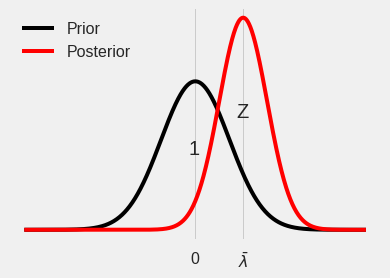
\includegraphics[width=0.5\textwidth]{correlations/plots/lambdapriorpost.png}
    \caption{Sketch of the prior (Eqn.~\ref{eqn:lambdaprior}) and posterior (Eqn.~\ref{eqn:lambdaposterior}) distributions for $\lambda$. Adding information shifts the distribution and reduces the width. \label{fig:lambdadistribs}}
    
  \end{center}
\end{figure}
%%%%%%%%%%%%%%%%%%%%%%%%%%%%%%%%%%%%%%%%%%%%%%%%%%%%%%%%%%%%%%%%%%%%%%

\subsection{Decorrelation}
We will now test out this formalism in the case of a ``perfect fit". This is one where the theory inputs to the fit are flexible enough to fit the data exactly. It is not a especially realistic situation in the context of PDF fits, but will serve as a useful foundation on which to model more complex situations. 

In this perfect fit $P(T|D)$ (Eqn.~\ref{eqn:ptd2}) is maximised when $T=D$, which corresponds to $\chi^2 = 0$. The data and theory are therefore fully correlated, and the expectation value, $E[\cdot]$, and covariance, $\Cov[\cdot]$, of the theory are
\be
\label{eq:perfectfit}
E[T] = D,\qquad \Cov[T] = \Cov[D] = C+S.
\ee
Looking back at the definition of $\bar{\lambda}$, we can see that after the fit $\bar{\lambda}=0$, and so Eqn.~\ref{eqn:lambdaposterior} is independent of $T$. The posterior for $\lambda$ has 
\be 
\label{eq:meanvarlam}
E[\lambda] =0,\qquad \Var[\lambda] = Z.
\ee
%%%%%%%%%%%%%%%%%%%%%%%%%%%%%%%%%%%%%%%%%%%%%%%%%%%%%%%%%%%%%%%%%%%%%
\begin{figure}[H]
  \begin{center}
      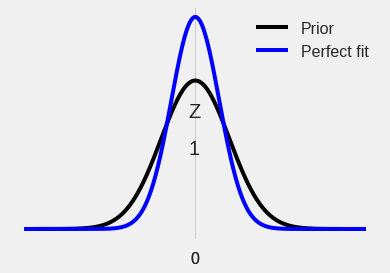
\includegraphics[width=0.5\textwidth]{correlations/plots/lambdaperfectfit.png}
    \caption{Sketch of the prior (Eqn.~\ref{eqn:lambdaprior}) and posterior (Eqn.~\ref{eqn:lambdaposterior}) distributions for $\lambda$ in the case of a perfect fit. The additional information from $D$ reduces the uncertainties but there is no shift as the theory fit the data exactly. \label{fig:lambdaperfect}}
   
  \end{center}
\end{figure}
%%%%%%%%%%%%%%%%%%%%%%%%%%%%%%%%%%%%%%%%%%%%%%%%%%%%%%%%%%%%%%%%%%%%%%
Fig.~\ref{fig:lambdaperfect} shows a sketch of the effect on the distribution of $\lambda$. What happens if we fit $T$ to $D$ and then use the results of this fit to make predictions for $T$? We can call this an ``autoprediction", because we are making predictions about the theory included in the fit itself. In effect this is like making theory predictions for another set of experimental results where the settings tie up exactly with those already included in the fit. In this scenario, the uncertainty is reduced as the experimental data have added information. Remembering that we can write $T(\lambda) = T + \lambda \beta$, we find
\be
\label{eq:perfectcovT}
\begin{split}
&E[T(\lambda)] = E[T]=D \\ &{\Cov}[T(\lambda)] 
= {\Cov}[T] + \Var[\lambda] \beta\beta^T = C+S+ZS.
\end{split}
\ee
There are three contributions to the covariance: the experimental uncertainty in the data, the theory uncertainty in the fit, and the theory uncertainty in the prediction. Note that the theory uncertainty in the prediction is reduced by a factor $Z={\rm Var}[\lambda]$, because of the correlation between this and the theory uncertainty in the fit. Note that:
\begin{itemize}
\item ignoring correlations amounts to setting $Z=1$ and we get ${\Cov}[T(\lambda)] = C + 2S$. This is the ``conservative prescription" of Chapter.~\ref{chapter:mhous}.
\item adopting the approach of \cite{Harland-Lang:2018bxd} and assuming full correlations amounts to setting $Z=0$ and we get ${\Cov}[T(\lambda)] = C + S$, so the conservative prescription double counts with respect to this.
\end{itemize}
In reality, the situation is somewhere between these two; we see a partial decorrelation due to the presence of experimental uncertainties.

To get a better sense of the size of decorrelation, let's consider a simple model where the experimental covariance matrix is diagonal and the theory uncertainty is fully correlated. Writing $\beta = s e$, where $s$ is the size of correlated theory uncertainty and $e^Te=1$, we have
\be
\label{eq:modelCS}
C = \sigma^2 \mathbb{I},\qquad S = s^2 e e^T,
\ee
where $\sigma$ is the per-point uncertainty. Then we can evaluate:
\be
\begin{split}
\label{eq:modelCplusSinv}
(C+S)^{-1} &= \frac{1}{\sigma^2}\left(1-\frac{s^2}{\sigma^2+s^2}e e^T\right); \\
Z &= (1+s^2/\sigma^2)^{-1}.
\end{split}
\ee
so we see that the extent of decorrelation depends on the ratio $s^2/\sigma^2$:
\begin{itemize}
\item as $\sigma^2/s^2 \to 0$ we tend to the case of no experimental uncertainties, as considered in \cite{Harland-Lang:2018bxd}, and $Z \to 0$.
\item as $s^2/\sigma^2 \to 0$, $Z \to 1$, which is the conservative prescription.
\end{itemize}
%%%%%%%%%%%%%%%%%%%%%%%%%%%%%%%%%%%%%%%%%%%%%%%%%%%%%%%%%%%%%%%%%%%%%
\begin{figure}[h]
  \begin{center}
      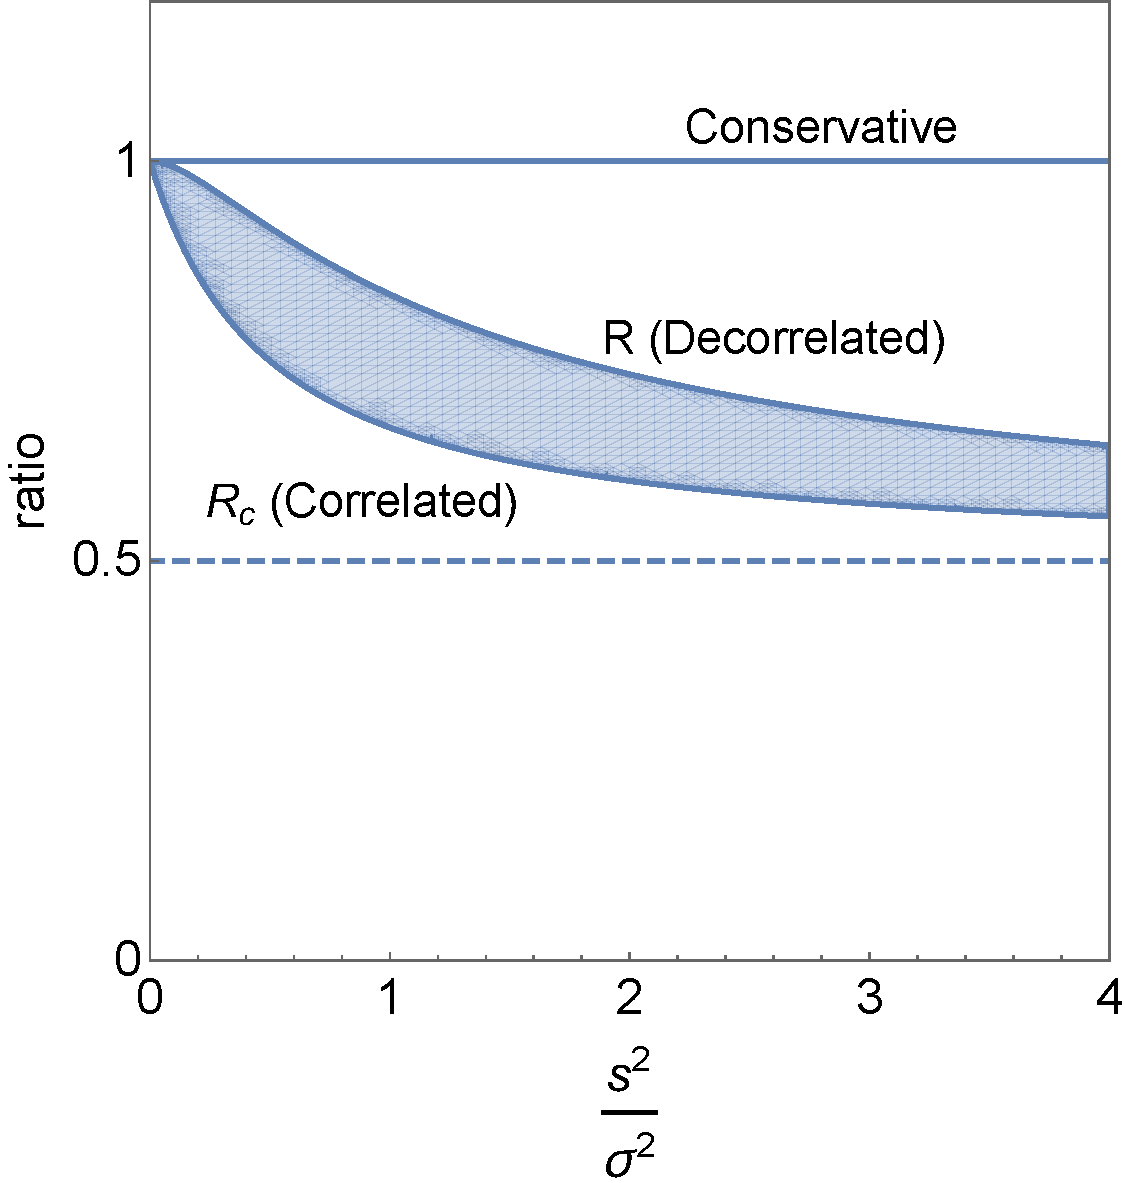
\includegraphics[width=0.5\textwidth]{correlations/plots/plot1.pdf}
    \caption{ For a perfect fit within the model Eqn.~\ref{eq:modelCS}.  Comparing the ratios to the conervative prescription of the decorrelated ($R$, Eqn.~\ref{eq:modelR}) and correlated ($R_c$, Eqn.~\ref{eq:modelRc}) autoprediction covariance matrices.  \label{fig:plot1}}
  \end{center}
\end{figure}
%%%%%%%%%%%%%%%%%%%%%%%%%%%%%%%%%%%%%%%%%%%%%%%%%%%%%%%%%%%%%%%%%%%%%%

Now consider the covariance matrix of autopredictions. In the conservative case this is $C + 2S$, which in the direction of $e$ is $\sigma^2 + 2s^2$. In any direction orthogonal to $e$ it is just $\sigma^2$ because there are no theory uncertainties in these directions. We can calculate the ratio of the true covariance matrix to the conservative one within the model in Eqn.~\ref{eq:modelCS}. This ratio is
\bea
R = \frac{e^T(C+S+ZS)e}{e^T(C+2S)e} &=& \frac{\sigma^2+(1+Z)s^2}{\sigma^2+2s^2}\nn\\
&=& 1-\frac{s^4}{\sigma^4+3\sigma^2 s^2 + 2s^4}\nn\\
&\sim&  \begin{cases}{1 -\smallfrac{ s^4}{\sigma^4} \qquad\mbox{for $s^2\ll\sigma^2 $;}}\\{ \half(1+\smallfrac{3\sigma^2}{2s^2})\qquad \mbox{for $s^2 \gg \sigma^2$.}}\end{cases} 
\label{eq:modelR}
\eea
We can see that
\begin{itemize}
\item when experimental uncertainties dominate then the theory uncertainties are almost entirely decorrelated. In this case the conservative prescription is almost exact; only a slight overestimate.
\item when theory uncertainties dominate then there is very little decorrelation, and the conservative prescription double counts the theory uncertainties.
\end{itemize}
When we're between these extremes, we can look at the difference between this ratio and that for the fully correlated case, which is
\bea
R_c = \frac{e^T(C+S)e}{e^T(C+2S)e} &=& 1 -\frac{s^2}{\sigma^2+2 s^2}\nn\\
&\sim& \begin{cases}{1 - \smallfrac{s^2}{\sigma^2} \qquad\mbox{for $s^2\ll \sigma^2$;}}\\{ \half(1+\smallfrac{\sigma^2}{2s^2})\qquad \mbox{for $s^2\gg\sigma^2 $.}}\end{cases} 
\label{eq:modelRc}
\eea
The two ratios are shown in Fig.~\ref{fig:plot1}. When $s^2/\sigma^2$ is small, the effects from decorrelation are the strongest. When $s^2= \sigma^2$, as is the case for many experiments in NNPDF fits, $R=\smallfrac{5}{6}$ and $R_c = \frac{2}{3}$, so the decorrelation result is half way between the fully correlated and conservative cases.


\section{Predictions from one-parameter fits}
\label{sec:p2}
In the previous section we considered a perfect fit, where after fitting $T=D$. Now we consider the slightly more realistic scenario, where the fit is not perfect, but the theory predictions, $T(\theta)$, only depend on a single parameter, $\theta$. This is a useful model because it captures the essence of the fitting problem but it is sufficiently simple that we will be able to solve it exactly. The $\chi^2$ (Eqn.~\ref{eqn:chi2}) will be minimised for some $\theta = \theta_0$, with variance $\Var [\theta]$. Once $\theta_0$ has been determined we can then make some predictions, $\Ttil(\theta_0)$, where the tilde denotes they are predictions for theories separate from the fit inputs. These predictions will have uncertainties proportional to $\Var [\theta]$. 

We have assumed that the uncertainties are Gaussian, and so they are differentiable. This means we can linearise $T(\theta)$ about $T(\theta_0) \equiv T_0$:
\be
\label{eq:Tlin}
T(\theta) = T_0 + (\theta-\theta_0)\Tdot_0 + \dots .
\ee
We want to determine the uncertainty in the fitted $\theta$, so we need to propagate the uncertainties in the data, $D$, and the theory, $T(\theta)$, into $\theta$. We can do this using the standard NNPDF approach (see Chapter ~\ref{chapter:background}) of generating pseudodata replicas, $D^{(r)}$, which are Gaussianly distributed about the actual data, $D$, with covariance $C+S$. More explicitly, we can define the average over replicas for any function, $F$, of the replicas as
\be
\label{eq:repav}
\langle F(D^{(r)})\rangle =  \smallfrac{1}{N_{\rm rep}}\sum_{r=1}^{N_{\rm rep}}F(D^{(r)}).
\ee
Then the replicas will satisfy
\be 
\label{eq:repavD}
\langle D^{(r)}\rangle \equiv D^{(0)}, \qquad \langle (D^{(r)}-D^{(0)})(D^{(r)}-D^{(0)})^T\rangle = C+S.
\ee
In the limit of $N_{rep} \to \infty$, $D^{(0)} \to D$, and for finite replicas $D^{(0)}$ differs from $D$ by an amount which tends to zero like $N_{rep}^{-1/2}$.

The fit proceeds by fitting a parameter replica, $\theta^{(r)}$, for each pseudodata replica, $D^{(r)}$, by minimising
\be
\label{eq:chi2rep}
\chi_r^2[\theta] = (T(\theta)-D^{(r)})^T(C+S)^{-1}(T(\theta)-D^{(r)}),
\ee
with respect to $\theta$. Using Eqn.~\ref{eq:Tlin}, this leads to 
 \be
\label{eq:arep}
\theta^{(r)} - \theta_0 = \frac{\Tdot_0^T(C+S)^{-1}(D^{(r)}-T_0)}{\Tdot_0^T(C+S)^{-1}\Tdot_0}.
\ee
Now $\theta_0 = \langle \theta^{(r)} \rangle$, so using the replica averages in Eqn.~\ref{eq:repavD} we find
\be
\label{eq:consistency}
\Tdot_0^T(C+S)^{-1}(D-T_0)=0,
\ee
so we can rewrite Eqn.~\ref{eq:arep} as
\be
\label{eq:arep2}
\theta^{(r)} - \theta_0 = \frac{\Tdot_0^T(C+S)^{-1}(D^{(r)}-D)}{\Tdot_0^T(C+S)^{-1}\Tdot_0}.
\ee
Using the fact that $C$ and $S$ are symmetric, 
\bea
\Var[\theta] &=& \langle(\theta^{(r)}-\theta_0)^2\rangle\nn\\
 &=& \frac{\Tdot_0^T(C+S)^{-1}\langle(D^{(r)}-D)(D^{(r)}-D)^T\rangle (C+S)^{-1}\Tdot_0}{(\Tdot_0^T(C+S)^{-1}\Tdot_0)^2}\nn\\
&=& (\Tdot_0^T(C+S)^{-1}\Tdot_0)^{-1}.
\label{eq:vara}
\eea
Note that:
\begin{itemize}
\item data points with a large dependence on $\theta$ have large $\Tdot_0$ and contribute more.
\item directions with large uncertainty, $(C+S)$, contribute less.
\end{itemize}
Now we have the uncertainty in the fitted parameter, $\theta$, we can find the fitting uncertainty. This is the covariance of $T(\theta)$ due to the experimental and theoretical uncertainties from fitting $\theta$. We will call this covariance matrix $X$. Using the fact that $E[T] = \langle T(\theta^{(r)})\rangle = T(\theta_0) = T_0$ and writing $T^{(r)} = T(\theta^{(r)})$,
\bea
X\equiv\Cov[T(\theta)] &=& \langle(T^{(r)}-T_0)(T^{(r)}-T_0)^T\rangle\label{eq:Xdef}\\
&=& \Tdot_0\langle(\theta^{(r)}-\theta_0)^2\rangle\Tdot_0^T\\
&=& \Tdot_0(\Tdot_0^T(C+S)^{-1}\Tdot_0)^{-1}\Tdot_0^T\label{eq:Xdef2}\\
&=& n(n^T(C+S)^{-1}n)^{-1}n^T,
\label{eq:Xdef3}
\eea
where in the last line we define $\Tdot_0 \equiv |\Tdot_0|n$, i.e. $n$ is a unit vector in the direction of $\Tdot_0$. We can see that $X$ depends only on the direction ($n$) of $\Tdot_0$, not its magnitude. Note that $X$ is singular and also that
\be
\label{eq:XsqeqX}
X = X(C+S)^{-1}X,
\ee
which will be useful later. Using Eqn.~\ref{eq:arep2} in Eqn.~\ref{eq:Tlin}, we can see that
\be
T^{(r)}-T_0 = X(C+S)^{-1}(D^{(r)}-D^{(0)}),
\label{eq:projection}
\ee
so $X(C+S)^{-1}$ projects the data replicas onto the theory replicas.

Now let's revisit the model for covariance matrices, Eqn.~\ref{eq:modelCS}. If we define the angle between the experimental uncertainties and the $\theta$ variation by $\cos \phi = n^T e$, we find that
\bea
\label{eq:denom}
n^T(C+S)^{-1}n &=& \frac{\sigma^2+s^2\sin^2\phi}{\sigma^2(\sigma^2+s^2)},\\
n^TXn &=& \frac{\sigma^2(\sigma^2+s^2)}{(\sigma^2+s^2\sin^2\phi)}.
\eea
Note that using any vector other than $n$ here gives 0. We can see that the effects from the theory uncertainty ($s$) depend on its degree of alignment with $n$, the direction of the parameter dependence. 
\begin{itemize}
\item For complete alignment, $\phi=0$ and the variance of $T$ in this direction is $(\sigma^2 + s^2)$.
\item When they are orthogonal, $\phi= \smallfrac{\pi}{2}$ and the variance is $\sigma^2$, so the theory uncertainty doesn't factor into the fitting.
\end{itemize}

\subsection{Autopredictions in a single parameter fit}
Now let's consider making autopredictions in this single parameter fit,
\be
\label{eq:autopred}
T(\theta,\lambda)=T(\theta)+\lambda\beta .
\ee
When fitting, we:
\begin{enumerate}
\item Maximise $P(T(\theta)|D)$ replica by replica to get $\{ \theta^{(r)} \}$.
\item Maximise $P(\lambda |T(\theta) D)$ replica by replica, using the values $\{ \theta^{(r)} \}$ from 1., to get  $\{ \lambda^{(r)} \}$.
\item Average over replicas to obtain the fitted results.
\end{enumerate}
For example, from Eqn.~\ref{eqn:lambdabardef} we can write
\be
\label{eq:lambdabarz}
E[\lambda] = \langle \bar{\lambda}(\theta^{(r)}) \rangle =  \overline\lambda(\theta_0) = \beta^T(C+S)^{-1}(D^{(0)}-T_0).
\ee
Now that in general $D \neq T_0$, the nuisance parameters can have non-zero expectation values, and this will contribute to the expectation value of the autopredictions:
\be
\label{eq:ET}
E[T(\theta,\lambda)] = \langle T(\theta^{(r)},\overline\lambda(\theta^{(r)})\rangle =  
T(\theta_0,\overline\lambda(\theta_0)) = T(\theta_0)+\overline\lambda_0\beta.
\ee
So the data give information on the theory uncertainty by inducing shifts in the autopredictions:
\be
\label{eq:shift}
\delta T(\theta_0) = \beta\beta^T(C+S)^{-1}(D^{(0)}-T(\theta_0)) = S(C+S)^{-1}(D^{(0)}-T(\theta_0)).
\ee
Recall that $n^T(C+S)^{-1}(D^{(0)}-T(\theta_0)) =0$ from Eqn.~\ref{eq:consistency}, so we only get non-zero shifts when $n$ and $e$ (the data and the theory) point in different directions. When they are parallel ($\theta =0$), the theory uncertainty is just absorbed into the fit.

Now let's look at the change in the uncertainty of the autopredictions relative to the original predictions. The variance of $\lambda$ has two independent contributions in this scenario:
\begin{enumerate}
\item the width of the posterior, $P(\lambda | T(\theta) D)$;
\item the fluctuation of $\lambda (\theta)$ due to changing $\theta$ over replicas.
\end{enumerate}
So we can write
\be
\label{eq:varlamdef}
\Var[\lambda] = E[(\lambda-\overline\lambda_0)^2] = E[(\lambda-\overline\lambda(\theta^{(r)})^2]+ \langle(\overline\lambda(\theta^{(r)})-\overline\lambda_0)^2\rangle.
\ee
It's easiest to first address these two contributions separately. The first term is analogous to that in Sec.~\ref{sec:p1}, and we can use the Sherman Morrison formula again to rewrite it:
\be
\begin{split}
\label{eq:Zdef2}
E[(\lambda-\overline\lambda(\theta^{(r)})^2] = Z &= (1 + \beta^T C^{-1}  \beta)^{-1} \\ &= 1-\beta^T(C+S)^{-1}\beta,
\end{split}
\ee
As for the second term, we can use the definitions of $\bar{\lambda}$ and $\bar{\lambda}_0$, and then Eqn.~\ref{eq:projection} to write
\bea
 \overline\lambda(\theta^{(r)})-\overline\lambda_0 &=& \beta^T(C+S)^{-1}(D^{(r)}-D^{(0)}-(T^{(r)}-T_0))\nn\\
&=& \beta^T(C+S)^{-1}(D^{(r)}-D^{(0)}-(\theta^{(r)}-\theta_0)\Tdot_0)\nn\\
&=& \beta^T(C+S)^{-1}(1-X(C+S)^{-1})(D^{(r)}-D^{(0)}).\label{eq:lamalgebra}
\eea
So we can then get
\bea
 \langle(\overline\lambda(\theta^{(r)})-\overline\lambda_0)^2\rangle &=&
\beta^T(C+S)^{-1}(1-X(C+S)^{-1})\langle(D^{(r)}-D^{(0)})(D^{(r)}-D^{(0)})^T\rangle\nn\\
&&\qquad\qquad \times(1-(C+S)^{-1}X)(C+S)^{-1}\beta\nn\\.
\eea
Then using Eqn.~\ref{eq:repavD} followed by Eqn.~\ref{eq:XsqeqX}:
\bea
 \langle(\overline\lambda(\theta^{(r)})-\overline\lambda_0)^2\rangle &=&\beta^T((C+S)^{-1}-2(C+S)^{-1}X(C+S)^{-1}\nn\\
&&\qquad +(C+S)^{-1}X(C+S)^{-1}X(C+S)^{-1})\beta
\label{eq:varlambar1}\\
&=&\beta^T(C+S)^{-1}\beta-\beta^T(C+S)^{-1}X(C+S)^{-1}\beta
\label{eq:varlambar2}
\eea
So overall 
\be
\label{eq:Zbardef}
\Var[\lambda] = 1 -\beta^T(C+S)^{-1}X(C+S)^{-1}\beta\equiv \Zbar.
\ee
We can see that $\bar{Z} \leq 1$ because $(C+S)^{-1}X(C+S)^{-1}$ is positive semidefinite, and noting that $\bar{Z} = Z + \langle(\overline\lambda(\theta^{(r)})-\overline\lambda_0)^2\rangle$, it is clear that $\bar{Z} \geq Z$. When $n=e$, so that the $\theta$ variation and the theory uncertainty are aligned, we get $\bar{Z} = Z$. So in summary
\be
\label{zbarbounds}
0<Z\leq\Zbar\leq 1.
\ee
In other words, there is more decorrelation in this constrained fit than in the perfect fit of Sec.~\ref{sec:p1}, because the fit uncertainty causes additional decorrelation. This is the second mechanism for decorrelation we have uncovered, on top of the decorrelation due to experimental uncertainties observed in Sec.~\ref{sec:p1}.

Finally we can use the model for uncertainties (Eqn.~\ref{eq:modelCS}) to show that
\be
\label{eq:Zbarmod}
\Zbar = \frac{\sigma^2 + s^2 \sin^2\phi}{\sigma^2+s^2}.
\ee
So, comparing this with the expression for $Z$ (Eqn.~\ref{eq:modelCplusSinv}), $\bar{Z} = Z$ when $\phi =0$, as expected, and $\bar{Z}=1$ when $\phi = \smallfrac{\pi}{2}$; here the data have no effect on the uncertainty, so we have total decorrelation.

Let's also calculate the covariance of autopredictions in the model. This is made up of two contributions:
\begin{enumerate}
\item the variation about $\bar{\lambda}$;
\item the fluctuations of the individual replicas in the fit.
\end{enumerate}
\bea
{\Cov}[T(\theta,\lambda)] &=& E[(\lambda-\lambdabar(\theta))^2]\beta\beta^T 
 + \Cov[T(\theta,\lambdabar(\theta)]\label{eq:covTsumx}\nn\\
&=& ZS 
 + \langle(T(\theta^{(r)},\lambdabar(\theta^{(r)})) -T(\theta_0,\lambdabar_0))^2 \rangle  \label{eq:covTsum}
\eea
Let's first calculate
\bea
T(\theta^{(r)},\lambdabar(\theta^{(r)}))-T(\theta_0,\lambdabar_0) &=& T(\theta^{(r)}) - T(\theta_0) + (\bar{\lambda}(\theta^{(r)}) - \bar{\lambda_0}) \beta \\
&=& X(C+S)^{-1}(D^{(r)}-D^{(0)}) \\ &&\qquad + \beta \beta^T (C+S)^{-1}(1-X(C+S)^{-1}) \qquad \qquad \\ && \qquad \times (D^{(r)}-D^{(0)}) \\
&=& [ X(C+S)^{-1} \\ && \qquad + S(C+S)^{-1}(1-X(C+S)^{-1}) ] \qquad \\ && \qquad \times  (D^{(r)}-D^{(0)}).
\eea
Now consider right multiplying the term in $[ \cdot ]$ by $\mathbb{I} = (C+S)(C+S)^{-1}$, and it can be shown that
\be
T(\theta^{(r)},\lambdabar(\theta^{(r)}))-T(\theta_0,\lambdabar_0) = (S+C(C+S)^{-1}X)(C+S)^{-1}(D^{(r)}-D^{(0)}).\label{eq:Tarep}
\ee
So, using Eqn.~\ref{eq:XsqeqX} to simplify the quadratic in $X$, the second term is
\bea
{\Cov}[T(\theta,\lambdabar)]&=&\langle(T(\theta^{(r)},\lambdabar(\theta^{(r)}))-T(\theta_0,\lambdabar_0))(T(\theta^{(r)},\lambdabar(\theta^{(r)}))-T(\theta_0,\lambdabar_0))^T\rangle\nn\\ 
&=& (S+C(C+S)^{-1}X)(C+S)^{-1}(S+X(C+S)^{-1}C)\nn\\ \qquad
&=&  S(C+S)^{-1}S + X - S(C+S)^{-1}X(C+S)^{-1}S. \qquad \qquad \label{eq:covTrlamr}
\eea
So the total covariance of autopredictions is
\bea
{\Cov}[T(\theta,\lambda)] &=& (S - S(C+S)^{-1}S) + (S(C+S)^{-1}S +X - S(C+S)^{-1}X(C+S)^{-1}S)\nn\\
&=& X + S - S(C+S)^{-1}X(C+S)^{-1}S \\
&=& X + \bar{Z} S. \label{eq:covTfit2}
\eea
This is the same as if we had assumed that $T(\theta)$ and $\lambda$ are uncorrelated, i.e. that
\be
{\Cov}[T(\theta,\lambda)] = {\Cov}[T] + \Var[\lambda] \beta\beta^T 
= X+\Zbar S.\label{eq:covTfit}
\ee
So we see that the cross correlations between $T(\theta)$ and $\lambda$ have cancelled.

We can use the model again to calculate the ratio of this covariance to the one given by the conservative prescription:
\bea
\Rbar &=& \frac{e^T(X+\Zbar S)e}{e^T(X+S)e}\nn\\
&=& 1 - \frac{s^4\cos^2\phi}{\sigma^2+ s^2}\frac{\sigma^2+s^2\sin^2\phi}{\sigma^2(\sigma^2+s^2)\cos^2\phi+s^2(\sigma^2+s^2\sin^2\phi)}\nn\\
&\sim&  \begin{cases}{1 -\smallfrac{ s^4}{\sigma^4} \qquad\qquad\mbox{for $s^2 \ll \sigma^2$;}}\\{ \sin^2\phi +\smallfrac{\sigma^2{\rm cot}^2\phi}{s^2}\qquad \mbox{for $s^2 \gg \sigma^2$.}}\end{cases} 
\label{eq:modelRbar}
\eea
\begin{itemize}
\item When the experimental uncertainties dominate, $\sigma^2 \gg s^2$  and there is almost total decorrelation, as before. The conservative prescription is a very good approximation.
\item When the theory uncertainties dominate, $s^2 \gg \sigma^2$, and the extent of decorrelation is $ \propto \sin^2 \phi$. If $n$ and $e$ are closely aligned this is small, but if they're orthogonal then fitting the data has no effect on the theory uncertainty, so we have total decorrelation. In that case the assumption of full correlation is a big underestimate. 
\end{itemize}
The ratio to the full correlation case is
\bea
\Rbar_c &=& \frac{e^TXe}{e^T(X+S)e}\nn\\
&\sim& \begin{cases}{1 - \smallfrac{s^2}{\sigma^2\cos^2\phi} \qquad\mbox{for $s^2 \ll \sigma^2$;}}\\{ \smallfrac{\sigma^2{\rm cot}^2\phi}{s^2}\qquad \mbox{for $s^2 \gg \sigma^2$.}}\end{cases} 
\label{eq:modelRbarc}
\eea
Fig.~\ref{fig:plot2} shows a comparison between these two. When $\phi$ is small, the limit of $\smallfrac{s^2}{\sigma^2}$ is reached much more slowly because it requires $s^2 \gg \sigma^2 \cot^2 \phi$.
%%%%%%%%%%%%%%%%%%%%%%%%%%%%%%%%%%%%%%%%%%%%%%%%%%%%%%%%%%%%%%%%%%%%%
\begin{figure}[h]
  \begin{center}
      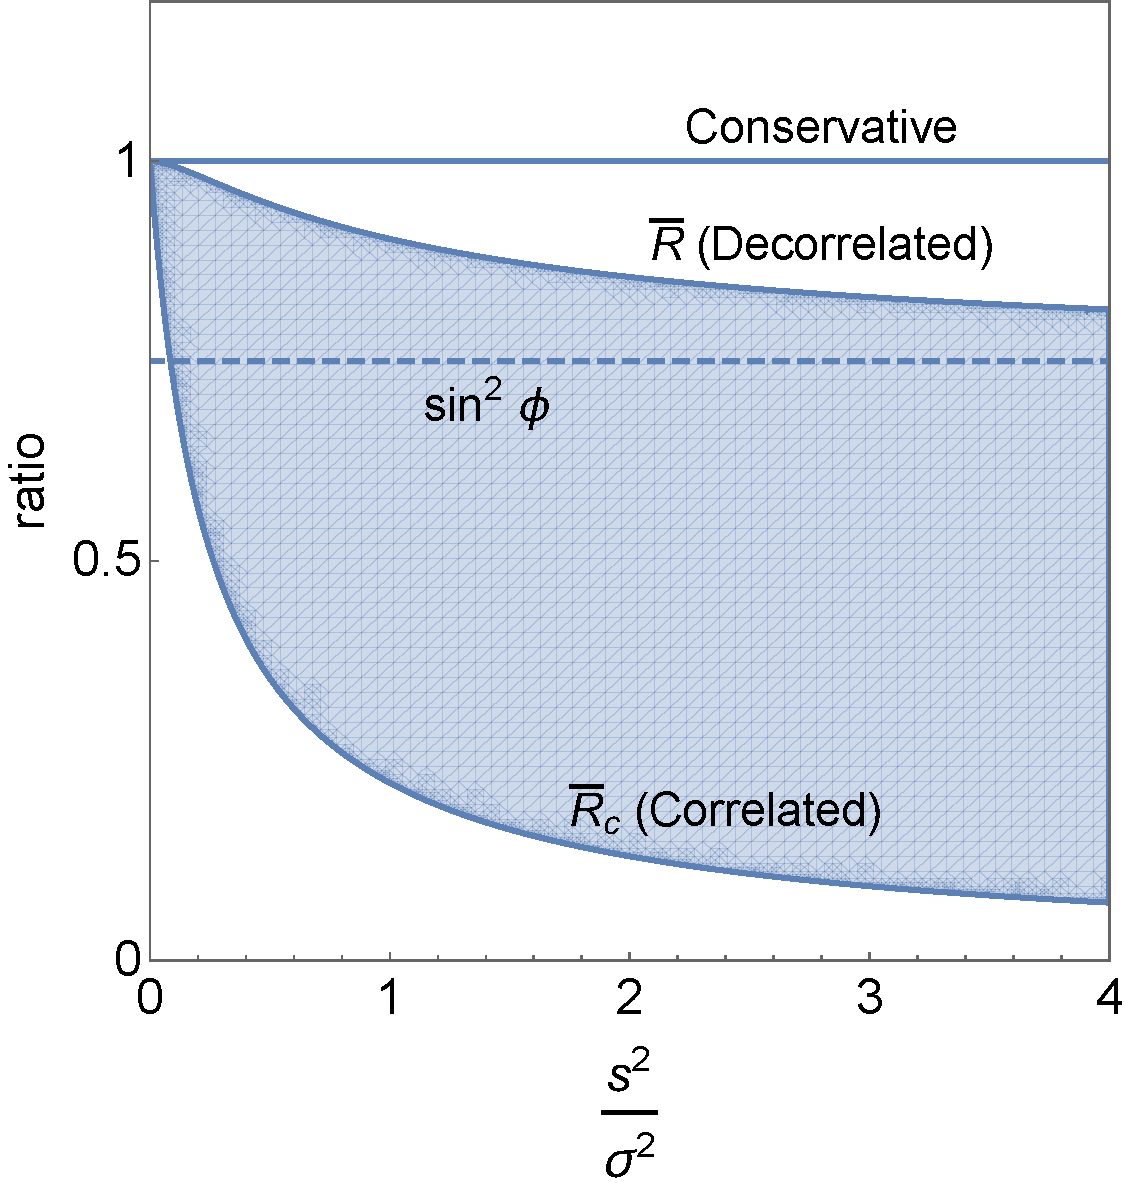
\includegraphics[width=0.5\textwidth]{correlations/plots/plot2.pdf}
    \caption{ For single parameter fit within the model Eqn.~\ref{eq:modelCS}.  Comparing the ratios to the conervative prescription of the decorrelated ($\Rbar$, Eqn.~\ref{eq:modelRbar}) and correlated ($\Rbar_c$, Eqn.~\ref{eq:modelRbarc}) autoprediction covariance matrices.  \label{fig:plot2}}
  \end{center}
\end{figure}
%%%%%%%%%%%%%%%%%%%%%%%%%%%%%%%%%%%%%%%%%%%%%%%%%%%%%%%%%%%%%%%%%%%%%%
\subsection{Correlated predictions}
Let's think about making predictions for other observables not in the fit. We denote these $\Ttil_I(\theta)$, $I=1,\ldots , \widetilde{N}$. They depend on the same $\theta$ parameter as the fitted predictions, $T_i(\theta)$, $i=1, \ldots , N$. There are two sources of uncertainty in $\Ttil_I(\theta)$:
\begin{enumerate}
\item that coming from the fit, i.e. the uncertainty in $\theta$ due to the experimental uncertainty in $D_i$ and the theory uncertainty in $T_i(\theta)$.
\item the theory uncertainty in $\Ttil_I(\theta)$ themselves.
\end{enumerate}

Source 1. is expressed via Eqn.~\ref{eq:vara}. We can write
\be
\label{eq:Tlin2}
\Ttil(\theta) = \Ttil_0 + (\theta-\theta_0)\Ttildot_0,
\ee
and use the shorthand notation $\Ttil^{(r)}\equiv\Ttil(\theta^{(r)})$. Then the covariance of $\Ttil_I(\theta)$ due to the uncertainty in $\theta$ is just like we found before for the autopredictions:
\bea
\Xtil\equiv\Cov[\Ttil(\theta)] &=& \langle(\Ttil^{(r)}-\Ttil_0)(\Ttil^{(r)}-\Ttil_0)^T\rangle\label{eq:Xtildef}\\
&=& \Ttildot_0\langle(\theta^{(r)}-\theta_0)^2\rangle\Ttildot_0^T
= \Ttildot_0(\Tdot_0^T(C+S)^{-1}\Tdot_0)^{-1}\Ttildot_0^T \qquad \qquad \label{eq:Xtildef2}.
%\\
%&=& \rtil\ntil(n^T(C+S)^{-1}n)^{-1}\ntil^T.
%\label{eq:Xtildef3}
\eea

Source 2. can be either correlated or uncorrelated with that in $T_i(\theta)$. Let's consider first the case where it is uncorrelated, for example if $\Ttil(\theta)$ are for a different type of observable to $T(\theta)$. Then we can associate with them a nuisance parameter, $\lambdatil$, which is uncorrelated with $\lambda$, and has the same prior as $\lambda$. This means we can write
\be
\Ttil(\theta,\lambdatil) =  \Ttil(\theta) + \lambdatil\betatil,\label{eq:uncor}
\ee
Here $\betatil_I$ give the size of the theory uncertainty in $\Ttil_I(\theta)$. We can proceed by finding the expectation value and covariance of the predictions:
\bea
E[\Ttil(\theta,\lambdatil)] &=& \Ttil(\theta_0),\label{eq:uncorpred}\\
\Cov[\Ttil(\theta,\lambdatil)]&=& \Cov[\Ttil(\theta)]+\Var[\lambdatil]\betatil\betatil^T 
= \Xtil + \Stil,\label{eq:uncorcov}
\eea
where 
\be
\Stil = \betatil\betatil^T,\label{eq:Stildef}
\ee
is the theory covariance matrix of predictions. What this shows us is that when the theory uncertainty is uncorrelated, we just add it in quadrature to the uncertainty due to $\theta$ in the fit. This matches the recommendations of the conservative prescription.

How about when $\Ttil(\theta)$ are fully correlated to $T(\theta)$? In this case $\lambdatil = \lambda$, and we already have the expectation value and covariance of $\lambda$ for the fit in Eqns.~\ref{eq:lambdabarz},\ref{eq:Zbardef}. So
\be
\label{eq:corpredmean}
E[\Ttil(\theta,\lambda)] = \Ttil(\theta_0) + \overline\lambda(\theta_0)\betatil,
\ee
and we get a shift in predictions analogous to the case of the autopredictions, i.e.
\bea
\label{eq:shiftpred}
\delta \Ttil(\theta_0) &=& \betatil\beta^T(C+S)^{-1}(D^{(0)}-T(\theta_0)) \\ &=& \Shat (C+S)^{-1}(D^{(0)}-T(\theta_0)).
\eea
Here 
\be
\Shat = \betatil\beta^T,\label{eq:Shatdef}
\ee
is the cross-correlated theory covariance matrix between $T(\theta)$ and $\Ttil(\theta)$. We can also define, in analogy to Eqn.~(\ref{eq:Xdef}) and Eqn.~(\ref{eq:Xtildef2}),
\be
\Xhat = \Ttildot_0(\Tdot_0^T(C+S)^{-1}\Tdot_0)^{-1}\Tdot_0^T\label{eq:Xhat},
\ee
and note the corresponding projective relations 
\be
\Xhat(C+S)^{-1}X=\Xhat,\qquad X(C+S)^{-1}\Xhat^T=\Xhat^T,\qquad \Xhat(C+S)^{-1}\Xhat^T=\Xtil \label{eq:XhatsqeqXtil} .
\ee
Following on from this, we can write
\be
\Ttil(\theta^{(r)})-\Ttil(\theta_0) = \Xhat (C+S)^{-1}(D^{(r)}-D^{(0)}),\label{eq:Ttilrep}
\ee
and so
\be
\Ttil(\theta^{(r)},\lambdabar(\theta^{(r)}))-\Ttil(\theta_0,\lambdabar_0) = (\Xhat+\Shat-\Shat(C+S)^{-1}X)(C+S)^{-1}(D^{(r)}-D^{(0)}),\label{eq:Ttilarep}
\ee
which leads us to the contribution from Source 2.:
\be
\Cov[\Ttil(\theta,\lambdabar(\theta)] =  \Shat (C+S)^{-1}\Shat^T + \Xtil - \Shat(C+S)^{-1}X(C+S)^{-1}\Shat^T.\label{eq:covTtilrlamr}
\ee

Then the full covariance of the predictions is the combination of Source 1. and Source 2. (using Eqn.~\ref{eq:Zdef2}):
\bea
{\Cov}[\Ttil(\theta,\lambda)] &=& E[(\lambda-\lambdabar(\theta))^2]\Stil 
 + \Cov[\Ttil(\theta,\lambdabar(\theta)]\label{eq:covTtilsumx}\\
&=& (1-\beta^T (C+S)^{-1} \beta)\Stil + \Shat (C+S)^{-1}\Shat^T + \Xtil \\ &&\qquad - \Shat(C+S)^{-1}X(C+S)^{-1}\Shat^T \\
&=& \Xtil + \Stil - \Shat(C+S)^{-1}X(C+S)^{-1}\Shat^T.\label{eq:covTtilfit2}\\
&=& \Xtil +\Zbar \Stil. \\
\eea

In summary, including correlations betwen the theory uncertainties in the fit and the predictions:
\begin{itemize}
\item shifts the central value of the prediction;
\item reduces the uncertainty of the prediction.
\end{itemize}
The fit gives information from $D$ about the theory uncertainties, leading to a more precise prediction. Note that all of the theory covariance matrices are positive semidefinite, and that
\be
\label{eq:possemdeftil}
0\leq \Shat^T(C+S)^{-1}\Shat \leq \Stil,
\ee
so ${\Cov}[\Ttil(\theta,\lambda)]$ is always reduced by the subtracted term in Eqn.~\ref{eq:covTtilfit2}, but will never be negative (which would be nonsensical in this context). 

We can understand a little more about the various theory covariance matrices by imagining we obtained some experimental measurements, $\widetilde{D}$, corresponding to predictions $\Ttil$. Then we could add these to the fit, and would get a new fitting theory covariance matrix with dimensions $(N+\widetilde{N})\times(N+\widetilde{N})$ and content
\be
\left(\begin{array}{cc}
S&\Shat\\
\Shat^T&\Stil\end{array}\right)
 =
\left(\begin{array}{cc}
\beta\beta^T&\beta\betatil^T\\
\betatil\beta^T&\betatil\betatil^T\end{array}\right).
\label{eq:covmatglobal}
\ee
Here the role of $\Shat$ and $\Shat^T$ as cross-correlation theory covariance matrices is clear. We can see that the theory uncertainties in the prediction are consistent with the theory uncertainties we would use when including observables in a fit, which makes sense in the comparison with the autopredictions case. 

\section{Correlated MHOUs in PDF fits}
\label{sec:p3}
In this section we add another layer of complexity to the model we are building up. Now the theory values, $T_i[f]$, depend on PDFs, $f$, which are determined in a global fit to the $N$ data points, $D_i$, with experimental covariance $C_{ij}$. The PDFs are then used to make $\widetilde{N}$ theory predictions, $\Ttil_I[f]$.

In a PDF fit there are many potential sources of theory uncertainty, but here we will consider MHOUs, computed with scale variation using a prescription from Chapter~\ref{chapter:mhous}. In this case $S_{ij}$ and $\Stil_{IJ}$ have many non-zero eigenvalues. We can describe them using $n$ nuisance parameters, $\lambda_\alpha$, $\alpha = 1, \dots , n$. Usually $n \ll N$, but we don't impose a limit on $n$ here. 

We will now find the expectation value and covariance of these nuisance parameters, and use those to find the shifts in predictions, and  the change in their uncertainties.

\subsection{Multiple nuisance parameters}
\label{subsec:p31}
Here we repeat the analysis of Sec.~\ref{subsec:nuis}, but for multiple nuisance parameters rather than just one. Each nuisance parameter is associated with a shift in theory value $T_i[f]\to T_i[f] + \lambda_\alpha\beta_{i,\alpha}[f]$, using summation notation for $\alpha$. Note that the $\beta_{i,\alpha}$ don't have to be mutually orthogonal. We pick a prior for each nuisance parameter the same as in Sec.~\ref{subsec:nuis}, i.e. 
\be
\label{eq:priorf}
P(\lambda|D)=P(\lambda) \propto \exp\big(-\half\lambda_\alpha\lambda_\alpha\big).
\ee
Once again we assume Gaussianity, and now instead of Eqn.~(\ref{eq:PTDl}) we get
\be
\label{eq:PTDlf}
P(T|D\lambda)\propto \exp\big(-\half(T[f]+\lambda_\alpha\beta_\alpha-D)^TC^{-1}(T[f]+\lambda_\alpha\beta_\alpha-D)\big).
\ee
We can marginalise over $\lambda_\alpha$ to get 
\be
\label{eq:marginalise2}
P(T|D) \propto\int d^n\lambda\, \exp\left(-\half[(T[f]+\lambda_\alpha\beta_\alpha-D)^TC^{-1}(T[f]+\lambda_\beta\beta_\beta-D)+\delta_{\alpha\beta}\lambda_\alpha\lambda_\beta]\right)\, .
\ee
The next step is to complete the square in the exponent. After some work, defining 
\be
\label{eq:zdefmat}
Z_{\alpha\beta} = (\delta_{\alpha\beta}+\beta_\alpha^TC^{-1}\beta_\beta)^{-1},
\ee
where the bracketed inverse is with respect to $\alpha$, $\beta$, and
\be
\label{eq:lambdabarf}
\overline{\lambda}_\alpha = Z_{\alpha\beta}\beta_\beta^TC^{-1}(D-T),
\ee
we end up with
\be
\label{eq:integrationf}
P(T|D)\propto\int d^n\lambda\, \exp\left(-\half(\lambda_\alpha-\overline{\lambda}_\alpha) Z_{\alpha\beta}^{-1}(\lambda_\beta-\overline{\lambda}_\beta) - \half\chi^2\right) \propto \exp(-\half\chi^2).
\ee
Note that $\chi^2$ in this expression is given by Eqn.~(\ref{eq:chisq}) but where $S = \beta_\alpha\beta^T_\alpha$. Note also the analogy between this and Eqn.~\ref{eq:margresult}. 

We can then use Bayes' Theorem to get the posterior distribution, 
\be
\label{eq:posteriorf}
P(\lambda|TD)\propto \exp\big(-\half(\lambda_\alpha-\overline{\lambda}_\alpha) Z_{\alpha\beta}^{-1}(\lambda_\beta-\overline{\lambda}_\beta)\big),
\ee
and from this the expectation and covariance of $\lambda_\alpha$ are
\be
\label{eq:meanvarlamf}
E[\lambda_\alpha] =\lambdabar_\alpha,\qquad E[(\lambda_\alpha-\lambdabar_\alpha)(\lambda_\beta-\lambdabar_\beta)] = Z_{\alpha\beta}.
\ee
If we write $\beta = e_\alpha \beta_\alpha$, such that $e_\alpha$ is a unit eigenvector of $Z_{\alpha \beta}$, then the corresponding eigenvalue is $z = (1+\beta^TC^{-1}\beta)^{-1})$. This means $0<z<1$ and so $Z_{\alpha\beta}$ is positive definite, therefore invertible. What's more, if all $z <1$ then $\delta_{\alpha\beta}-Z_{\alpha\beta}$ is also positive definite. We can view $Z_{\alpha\beta}$ as the ``decorrelation matrix", upgrading it from the decorrelation coefficient from Sec.~\ref{subsec:nuis} as there are now many sources of uncertainty. 

We can write, in analogy with before,
\be
\label{eq:zdefmat2}
Z_{\alpha\beta} = \delta_{\alpha\beta}-\beta_\alpha^T(C+S)^{-1}\beta_\beta,
\ee
which allows us to rewrite $\overline{\lambda}_\alpha$, using $(1-(C+S)^{-1}S)C^{-1} = (C+S)^{-1}$, as
\be
\label{eq:lambdabarfx}
\overline{\lambda}_\alpha = \beta_\alpha^T(C+S)^{-1}(D-T[f]).
\ee

\subsection{Fitting PDFs with fixed parametrisation}
\label{subsec:p32}
Now we can use the previous section's results in the context of a PDF fit with MHOUs. In this section, we consider a fixed parametrisation of PDFs, like that adopted by, for example MSHT, CTEQ and ABM. Here the PDFs, $f(\theta)$, depend on $m$ parameters, $\theta_p$, $p=1, \dots , m$, where $m < N$ such that the data are able to determine all the parameters through $\chi^2$ minimisation. We will move on to the somewhat different case of PDFs with neural networks (unsurprisingly relevant to NNPDF) in the next section.

We adopt the same approach as in Sec.~\ref{sec:p2}, but fitting $m$ parameters, $\theta_p$, rather than a single one, $\theta$. Writing the PDF that minimises the $\chi^2$ as $f(\theta^0)\equiv f_0$, and using the notation $T_0\equiv T(\theta^0)$, $T_p\equiv \partial T(\theta^0)/\partial\theta_p^0$ with summation convention for $p$, we can linearise $T(\theta)$ as
\be
\label{eq:Tlinf}
T(\theta) = T_0 + (\theta_p-\theta_p^0)T_p + \dots .
\ee
Minimising this with respect to $\theta^p$, we find
\be
\label{eq:arep2f}
\theta^{(r)}_p - \theta^0_p = (T_p^T(C+S)^{-1}T_q)^{-1}T_q^T(C+S)^{-1}(D^{(r)}-D),
\ee
where the inverse of the left section is with respect to $p,q$. So
\bea
\Cov_{pq}[\theta] &=& \langle(\theta^{(r)}_p-\theta_p^0)(\theta^{(r)}_q-\theta_q^0)\rangle\nn\\
&=& (T_p^T(C+S)^{-1}T_q)^{-1}.
\label{eq:varaf}
\eea
To find $X$, we can separate out the magnitude and direction of $T_p$ by writing $T_p = |T_p|n_p$, where $n_p$ are (not necessarily orthogonal) unit vectors. Then Eqn.~\ref{eq:Xdef3} becomes
\be
X\equiv\Cov[T[f]] = n_p(n_p^T(C+S)^{-1}n_q)^{-1}n_q^T.
\label{eq:Xdeffpq}
\ee
Note that $X(C+S)^{-1}$ still projects the data replicas onto the theory replicas, and the projective relation for $X$ still holds. 

\subsubsection{Autopredictions}
First consider the autopredictions, $T(f,\lambda)\equiv T[f]+\lambda_\alpha\beta_\alpha$. We can see that the results from Sec.~\ref{sec:p2} still hold. In particular, the central values of $\overline{\lambda}_\alpha$ are given by Eqn.~\ref{eq:lambdabarfx}, and
the shifts (Eqn.~\ref{eq:shift}) are now
\be
\label{eq:shiftmult}
\delta T[f] = \beta_\alpha\beta_\alpha^T(C+S)^{-1}(D^{(0)}-T[f_0]) = S(C+S)^{-1}(D{(0)}-T[f_0]).
\ee
The covariance of $\lambda$ becomes an equation for the decorrelation matrix rather than a decorrelation coefficient:
\be
\label{eq:Zbardefab}
\Cov_{\alpha\beta}[\lambda] = \delta_{\alpha\beta} -\beta_\alpha^T(C+S)^{-1}X(C+S)^{-1}\beta_\beta\equiv \Zbar_{\alpha\beta}.
\ee
Like before, both $\Zbar_{\alpha\beta}$ and $\delta_{\alpha\beta}-\Zbar_{\alpha\beta}$ are positive semidefinite, so all eigenvalues of $\Zbar_{\alpha\beta}$ lie between zero and one. 

The covariance of the autopredictions then becomes
\be
{\Cov}[T(f,\lambda)] = X+\beta_\alpha\Zbar_{\alpha\beta}\beta_\beta^T = X + S - S(C+S)^{-1}X(C+S)^{-1}S.\label{eq:covTfitf}
\ee

\subsubsection{Predictions for new observables}
Now consider true predictions for new observables. The shifts (Eqn.~\ref{eq:shiftpred}) can be written
\be
\label{eq:shiftpredf}
\delta \Ttil[f] = \betatil_\alpha\beta_\alpha^T(C+S)^{-1}(D^{(0)}-T[f_0]) = \Shat (C+S)^{-1}(D^{(0)}-T[f_0]),
\ee
where we have defined $\Shat = \betatil_\alpha\beta_\alpha^T$. 

If the predictions are fully correlated, then $\Ttil(f,\lambda)=\Ttil[f]+\lambda_\alpha\betatil_\alpha$ and
\be
{\Cov}[\Ttil(f,\lambda)]
= \Xtil + \betatil_\alpha\Zbar_{\alpha\beta}\betatil_\beta^T = \Xtil + \Stil - \Shat(C+S)^{-1}X(C+S)^{-1}\Shat\label{eq:covTtilfitf},
\ee
where $\Stil = \betatil_\alpha\betatil_\alpha^T$. Finally, we have 
\be
\Xtil\equiv\Cov[\Ttil[f]] = \Ttil_p(T_p^T(C+S)^{-1}T_q)^{-1}\Ttil_q^T.
\label{eq:Xtildeff}
\ee

\subsection{Fitting NNPDFs}
In NNPDF we don't use a fixed parametrisation, but instead have a neural network with a very large number of parameters, in general greater than the number of data points. Here the ability to overfit is a danger, so we adopt a cross-validation procedure when finding the optimal $\chi^2$ (see Chapter \ref{chapter:background}). This means that when fitting each data replica, $D^{(r)}$, the $\chi^2$ is not exactly minimised; there is random noise in the system which amounts to a ``functional uncertainty"~\cite{Ball:2014uwa}. We will see in this section that this is responsible for a third mechanism of decorrelation, on top of those due to the experimental uncertainties and the loss of information in the fitting process.

The fact that Eqn.~\ref{eq:chi2rep} is not exactly minimised makes the analytical approach imprecise, and while in general the results in Sec.~\ref{subsec:p31} are valid, the exact relations for the fitted parameters (e.g. Eqn.~\ref{eq:arep2f}) and subsequent results do not hold. We are still able to use the PDF replicas compute, for example
\be
X\equiv\Cov[T[f]] = \langle (T^{(r)} - T^{(0)}) (T^{(r)} - T^{(0)})^T\rangle,
\label{eq:Xdefgen}
\ee
where $T^{(r)}\equiv T[f^{(r)}]$, and $T^{(0)}\equiv \langle T^{(r)}\rangle$. However, the projective relation for $X$ is no longer satisfied, and now $X(C+S)^{-1}$ doesn't project the data replicas on to the theory replicas.

The data and theory replicas no longer have an analytic connection, so we have to look instead at their correlations, which we can explicitly compute as 
\be
Y\equiv\Cov[T[f],D] = \langle (T^{(r)} - T^{(0)}) (D^{(r)} - D^{(0)})^T\rangle.
\label{eq:Ydefgen}
\ee
Note that $Y$ is in general not symmetric. In the case of a fixed parametrisation, such as in the previous section, then using Eqn.~\ref{eq:projection} and Eqn.~\ref{eq:repavD} we find $Y=Y^T=X$.

We will now redetermine the covariance of the nuisance parameters, then the autopredictions, and finally the external predictions. This time results will be in terms of $C$, $S$, $X$ and $Y$.

\subsubsection{Covariance of nuisance parameters}
Starting with
\be
\label{eq:lambdabarfxrep}
\overline{\lambda}^{(r)}_\alpha = \beta_\alpha^T(C+S)^{-1}(D^{(r)}-T^{(r)}),
\ee
we can compute
\begin{eqnarray}
\langle(\lambdabar_\alpha^{(r)}-\lambdabar_\alpha^{(0)})(\lambdabar_\beta^{(r)}-\lambdabar_\beta^{(0)})\rangle
&=& \beta_\alpha^T (C+S)^{-1}(C+S+X-Y-Y^T) \qquad \\ && \qquad \times (C+S)^{-1} \beta_\beta,\nn\\
&=& \beta_\alpha^T (C+S)^{-1}\beta_\beta + \beta_\alpha^T(X-Y-Y^T) \qquad \\ && \qquad \times  (C+S)^{-1} \beta_\beta,\label{eq:covlambdagen}
\end{eqnarray}
so
\be
\label{eq:Zbardefgen}
\Cov_{\alpha\beta}[\lambda] = \delta_{\alpha\beta} +\beta_\alpha^T(C+S)^{-1}(X-Y-Y^T)(C+S)^{-1}\beta_\beta\equiv \Zbar_{\alpha\beta}.
\ee
Note that when $X=Y=Y^T$ we get back Eqn.~\ref{eq:Zbardefab}. Also, although $\Zbar_{\alpha\beta}$ is still positive semidefinite, the eigenvalues are not bounded above by one any more, as $Y + Y^T$ is not generally positive definite. This means the presence of functional uncertainty can add another decorrelation effect which can be large enough to actually increase the theoretical uncertainties!

\subsubsection{Covariance of autopredictions}
The shifts in the autopredictions are still given by Eqn.~\ref{eq:shiftmult}, but the covaraince of autopredictions isn't the same. First note that
\bea
\label{eq:Talgebra}
T^{(r)} + \overline{\lambda}_\alpha^{(r)}\beta_\alpha &=& T^{(r)} + S(C+S)^{-1}(D^{(r)}-T^{(r)}) \\ &=&  C(C+S)^{-1}T^{(r)}  + S(C+S)^{-1}D^{(r)},
\eea
so
\begin{eqnarray}
\label{eq:covTbarx}
\Cov[T + \overline{\lambda}_\alpha\beta_\alpha] &=& C(C+S)^{-1}X(C+S)^{-1}C+S(C+S)^{-1}S \nn\\
&&\qquad+ C(C+S)^{-1}Y(C+S)^{-1}S \nn\\
&&\qquad+ S(C+S)^{-1}Y^T(C+S)^{-1}C. \nn\\
\end{eqnarray}
Then we can find the covariance matrix of predictions
\begin{eqnarray}
P\equiv\Cov[T(f,\lambda)] &=&\beta_\alpha Z_{\alpha\beta}\beta_\beta^T + \Cov[T + \overline{\lambda}_\alpha\beta_\alpha]\nn\\
&=& S+C(C+S)^{-1}X(C+S)^{-1}C \nn\\
&&\qquad+ C(C+S)^{-1}Y(C+S)^{-1}S \nn\\
&&\qquad+ S(C+S)^{-1}Y^T(C+S)^{-1}C \label{eq:covTfitfun}\\
&=&X +  \beta_\alpha \Zbar_{\alpha\beta}\beta_\beta^T - (X-Y)(C+S)^{-1}S \nn\\
&&\qquad- S(C+S)^{-1}(X-Y^T) \label{eq:covTfitfun2}.
\end{eqnarray}
Note again that when the functional uncertainty is zero, $X=Y=Y^T$ and we get back Eqn.~\ref{eq:covTfitf}. 

Now let's think about the case when the functional uncertainty is large. Then the theory replicas are almost totally uncorrelated with the data replicas, so $Y$ is much smaller than $C+S$ and $X$. In that situation 
\be
P \sim P_{\rm sim} =  S+C(C+S)^{-1}X(C+S)^{-1}C\label{eq:covTfitfunapprox},
\ee 
which is a little below the conservative result, $P_{\rm con}=X+S$. 

Revisiting the model (Eqn.~\ref{eq:modelCS}) a final time, we can look explicitly at the relative sizes of these. Using $X= x^2 nn^T$ for a unit vector, $n$, satisfying $e^Tn\equiv\cos\phi$. Then the ratio to the conservative result is
\bea
\Rbar_{\rm sim} &=& \frac{e^T(S+C(C+S)^{-1}X(C+S)^{-1}C)e}{e^T(S+X)e}\nn\\
&=& 1 - \frac{s^2(s^2+2\sigma^2)x^2\cos^2\phi}{(s^2+\sigma^2)^2(s^2+x^2\cos^2\phi)}\nn\\
&\sim&  \begin{cases}{1 -\smallfrac{ 2s^2}{\sigma^2} \qquad\qquad\mbox{for $s^2 \ll \sigma^2$ or $x^2$;}}\\{1-\smallfrac{x^2\cos^2\phi}{s^2}\qquad \mbox{for $s^2 \gg \sigma^2$ or $x^2$.}}\end{cases} 
\label{eq:modelRbarapprox}
\eea
Fig.~\ref{fig:plot3} shows a plot of this ratio. If $\sigma$ and $x$ are of similar size then $\Rbar_{\rm sim}$ always remains close to one, and there is almost total decorrelation, regardless of whether $s$ is small or large.
%%%%%%%%%%%%%%%%%%%%%%%%%%%%%%%%%%%%%%%%%%%%%%%%%%%%%%%%%%%%%%%%%%%%%
\begin{figure}[h]
  \begin{center}
      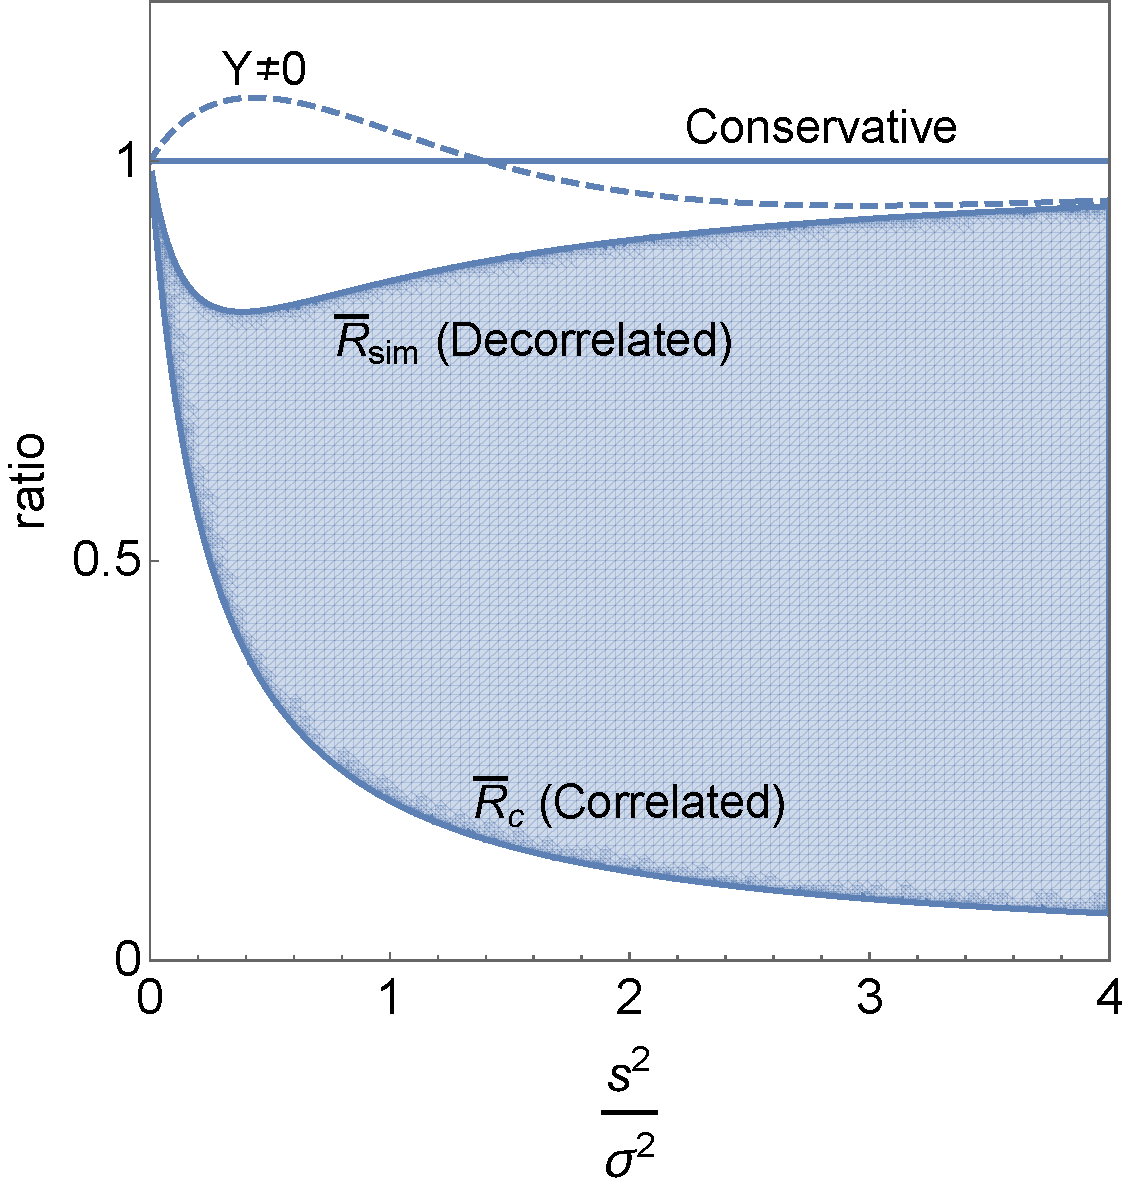
\includegraphics[width=0.5\textwidth]{correlations/plots/plot3.pdf}
    \caption{ For neural network fit within the model Eqn.~\ref{eq:modelCS}.  Comparing the ratios to the conervative prescription of the simplified decorrelated ($\Rbar_{\rm sim}$, Eqn.~\ref{eq:modelRbarapprox}) and correlated ($\Rbar_c$, Eqn.~\ref{eq:modelRbarc}) autoprediction covariance matrices.  \label{fig:plot3}}
  \end{center}
\end{figure}
%%%%%%%%%%%%%%%%%%%%%%%%%%%%%%%%%%%%%%%%%%%%%%%%%%%%%%%%%%%%%%%%%%%%%%
The effect when $Y \neq 0$ is also sketched. We understand that this will be modest, since the difference between $P_{\rm sim}$ and $P$ is small for both small and large $S$. However, we can get a slight over-decorrelation such that the true result actually goes slightly above the uncorrelated (conservative) result. What's more, this is in a region of relative uncertainties which is occupied by many datasets in current NNPDF fits. 

\subsubsection{Covariance of predictions for new observables}
Finally, consider predictions for new observables. The shifts are given by Eqn.~\ref{eq:shiftpredf}, and the covariance is
\begin{eqnarray}
\Ptil\equiv{\Cov}[\Ttil(f,\lambda)]
&=& \betatil_\alpha Z_{\alpha\beta}\betatil_\beta^T + \Cov[\Ttil + \overline{\lambda}_\alpha\betatil_\alpha]\nn\\
&=& \Xtil + \Stil + \Shat(C+S)^{-1}(X-Y-Y^T)(C+S)^{-1}\Shat^T  \nn\\
&&\qquad -(\Xhat-\Yhat)(C+S)^{-1}\Shat^T \nn\\
&&\qquad -\Shat(C+S)^{-1}(\Xhat^T-\Yhat^T) \label{eq:covTtilfitfun}\\
&=&\Xtil +  \betatil_\alpha \Zbar_{\alpha\beta}\betatil_\beta^T - (\Xhat-\Yhat)(C+S)^{-1}\Shat^T \nn\\
&&\qquad - \Shat(C+S)^{-1}(\Xhat^T-\Yhat^T) \label{eq:covTtilfitfun2}.
\end{eqnarray}
Note that we have defined the additional relations:
\begin{eqnarray} 
\Xtil&\equiv&\Cov[\Ttil[f]] = \langle (\Ttil^{(r)} -\Ttil^{(0)}) (\Ttil^{(r)} - \Ttil^{(0)})^T\rangle\label{eq:Xtildefgen},\\
\Xhat&\equiv&\Cov[\Ttil[f],T[f]] = \langle (\Ttil^{(r)} -\Ttil^{(0)}) (T^{(r)} - T^{(0)})^T\rangle\label{eq:Xhatdefgen},\\ 
\Yhat&\equiv&\Cov[\Ttil[f],D] = \langle (\Ttil^{(r)} -\Ttil^{(0)}) (D^{(r)} - D^{(0)})^T\rangle.
\end{eqnarray}
Again, we get the fixed parametrisation result when both $Y=Y^T=X$ and $\Yhat = \Xhat$. When there is a large functional uncertainty, $Y$ and $\Yhat$ are both small, and so
\bea
\Ptil_{\rm sim} &=&  \Xtil+\Stil + \Shat(C+S)^{-1}X(C+S)^{-1}\Shat^T \nn\\
&&\qquad -  \Xhat(C+S)^{-1}\Shat^T-\Shat(C+S)^{-1}\Xhat^T, \label{eq:covTtilfitfunapprox}
\eea 
which we expect to be close to the conservative predictions, $\Ptil_{\rm con}\equiv\Xtil+\Stil$.

\section{Numerical results}
\label{sec:p4}
Still with us? In this section we will apply all the results we worked up to in Sec.~\ref{sec:p3}. We have seen that in a realistic NNPDF fit, the shifts and uncertainties are much more complicated than the ones in the toy models (Secs.~\ref{sec:p1} and \ref{sec:p2}). This is due to
\begin{enumerate}
\item multiple nuisance parameters rather than just one;
\item functional uncertainty in the PDFs, i.e. the PDF parameters are not uniquely fixed.
\end{enumerate}
We showed that as well as the covariance matrix of theories, $X_{ij}$, we also need to compute the covariance between the theories and the data, $Y_{ij}$. Here we compute both of these and use them to generate autopredictions and then genuine predictions, where the effect of correlations is included.

We start by computing $X$ and $Y$. We use as a baseline the NNPDF3.1 NLO global fit with 9 point MHOUs which was generated in Chapter \ref{chapter:mhous}. This includes 2819 data points, split up into 5 processes. We use 1000 replicas because 100 replicas is insufficient to reliably calculate $Y$. This is because it is small due to large numerical cancellations. The only alteration we make to the fit is to drop the imposition of positivity at the data replica level, which was enforced in Ref.~\cite{Ball:2017nwa}. This is because imposing positivity skews the pseudodata generation and makes their distributions nongaussian. This makes negligible difference to the fit outcome, but can have an effect on the calculation of $Y$. Additionally, we are careful to distinguish between $D_i$ and $D_i^{(0)}$; they will be equal in the limit of infinite replicas and where the positivity condition has been dropped, but otherwise they differ slightly. As a final measure we employ a bootstrap method when calculating $Y$, resampling 1000 sets of 500 out of the 1000 total replicas.
%%%%%%%%%%%%%%%%%%%%%%%%%%%%%%%%%%%%%%%%%%%%%%%%%%%%%%%%%%%%
\begin{figure}[h]
    \begin{center}
    \makebox{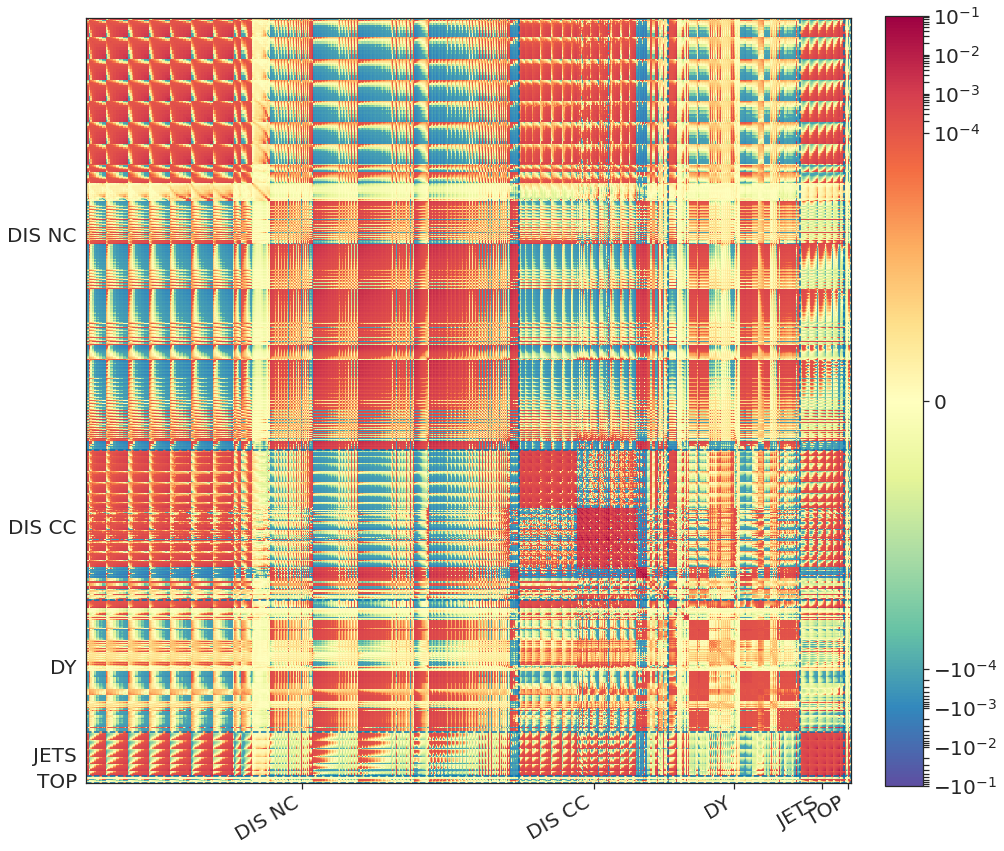
\includegraphics[width=0.45\columnwidth]{correlations/plots/X_covmat_cutscale.png}}
\makebox{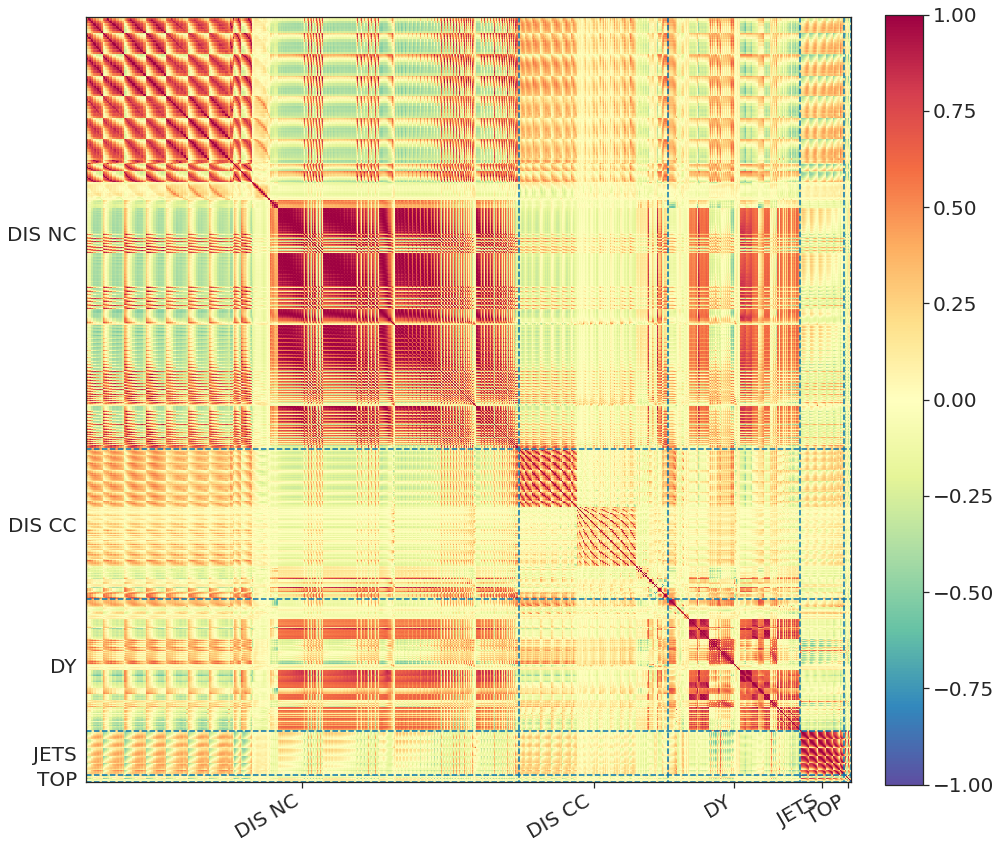
\includegraphics[width=0.45\columnwidth]{correlations/plots/Xcorrmat.png}}
    \end{center}
  \vspace{-0.55cm}
  \caption{The covariance matrix of PDF uncertainties, $X_{ij}$, normalised to the theoretical predictions $T^{(0)}_i$  (left), and the correlation matrix $X_{ij}/\sqrt{X_{ii}X_{jj}}$ (right). The order of datasets is given more explicitly in Fig.~\ref{fig:} below.}
  \label{fig:X}
\end{figure}
%%%%%%%%%%%%%%%%%%%%%%%%%%%%%%%%%%%%%%%%%%%%%%%%%%%%%%%%%%%%

The results for $X$ and $Y$ are shown in Figs.~\ref{fig:X} and \ref{fig:Y}, respectively. For each we show a heatmap normalised to theory, and the corresponding correlation matrix. The off-diagonal elements of $X$ are almost as large as the diagonal elements, demonstrated by strong correlations in the correlation matrix. These in turn come from strong theory correlations, especially in the nearby bins of the same experiment, but also for points from different processes at similar scales. 
%%%%%%%%%%%%%%%%%%%%%%%%%%%%%%%%%%%%%%%%%%%%%%%%%%%%%%%%%%%%
\begin{figure}[h]
    \begin{center}
    \makebox{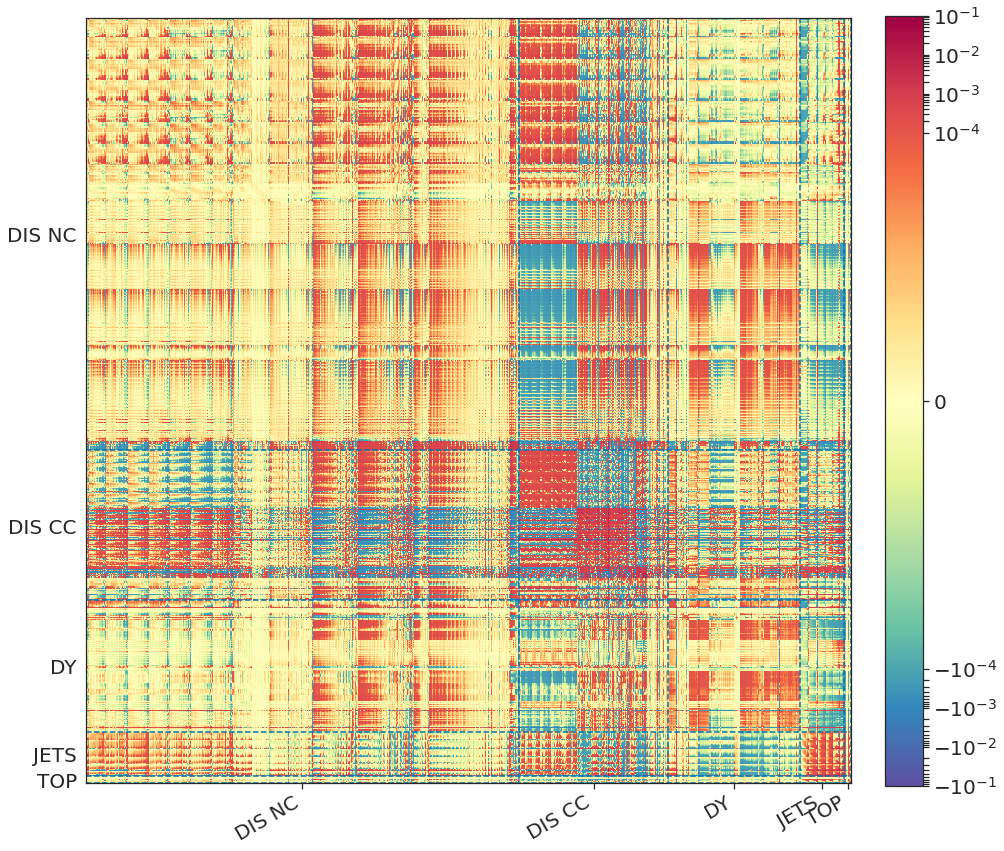
\includegraphics[width=0.45\columnwidth]{correlations/plots/Y_covmat_cutscale.png}}    
    \makebox{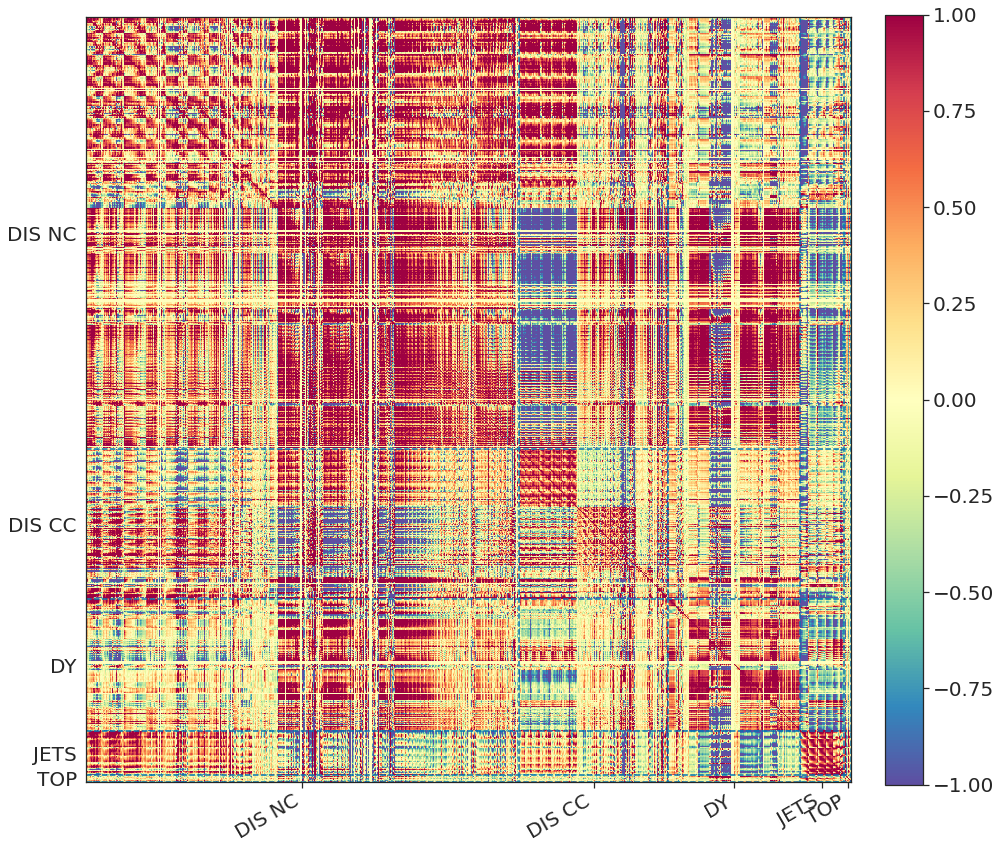
\includegraphics[width=0.45\columnwidth]{correlations/plots/Ycorrmat.png}}
    \end{center}
  \vspace{-0.55cm}
  \caption{The cross-covariance matrix of PDF uncertainties and data uncertainties, $Y_{ij}$, normalised to the theoretical predictions $T^{(0)}_i$  (left), and the correlation matrix $Y_{ij}/\sqrt{Y_{ii}Y_{jj}}$ (right).}
  \label{fig:Y}
\end{figure}
%%%%%%%%%%%%%%%%%%%%%%%%%%%%%%%%%%%%%%%%%%%%%%%%%%%%%%%%%%%%

$Y$ is clearly not symmetric, which is a result of the fit not being exact. There are some elements with large correlations across processes, although most of the elements of $Y$ are smaller than the corresponding ones in $X$. This is despite the fact that the data replica fluctuations are generally an order of magnitude larger than the theory replica fluctuations. This demonstrates the extent of decorrelation due to functional uncertainty.
%%%%%%%%%%%%%%%%%%%%%%%%%%%%%%%%%%%%%%%%%%%%%%%%%%%%%%%%%%%%
\begin{figure}[h]
    \begin{center}
    \makebox{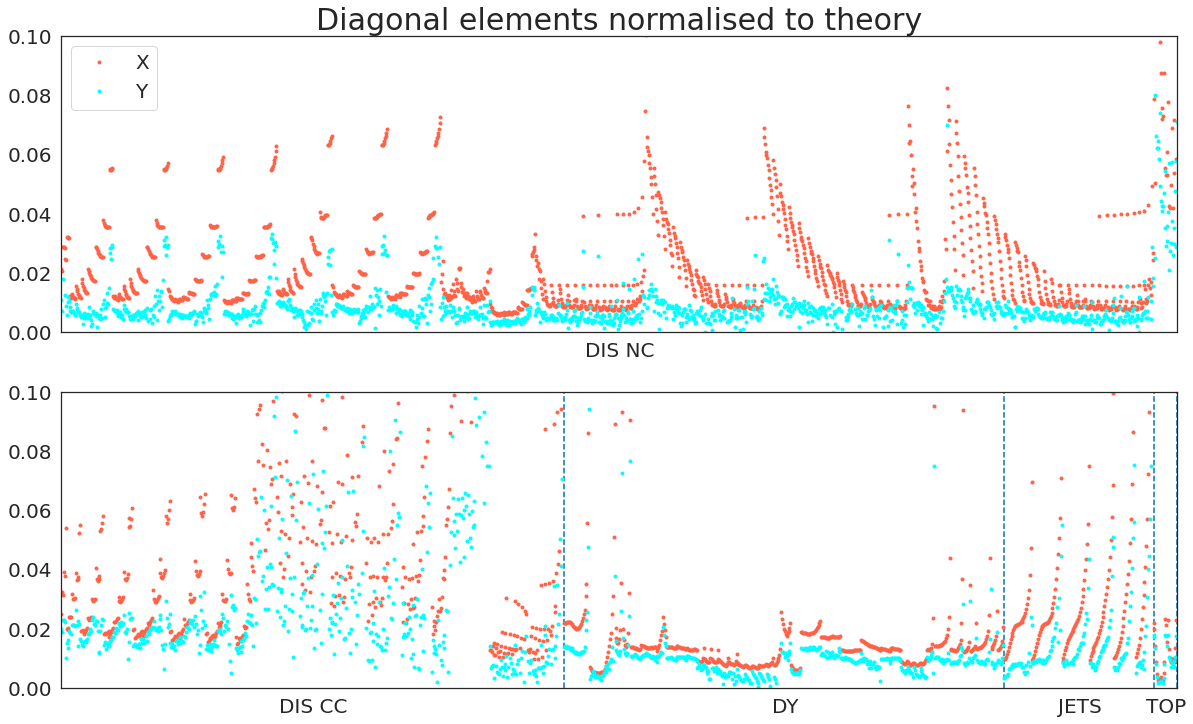
\includegraphics[width=0.99\columnwidth]{correlations/plots/diagxy.png}}
    \end{center}
  \vspace{-0.55cm}
  \caption{The diagonal elements of the matrices $X$ (in blue) and $Y$ (in orange), normalised to the theoretical predictions $T^{(0)}_i$.}
  \label{fig:XnYdiag}
\end{figure}
%%%%%%%%%%%%%%%%%%%%%%%%%%%%%%%%%%%%%%%%%%%%%%%%%%%%%%%%%%%%
Looking especially at the diagonal elements (Fig.~\ref{fig:XnYdiag}), $Y_{ii}$ are smaller than $X_{ii}$, showing that a given theory prediction is not well correlated to a single data point, because correlations to other data points in the fit are strong. This means we expect that ignoring $Y$'s contribution and hence using $P_{sim}$ rather than $P$ (Eqn.~\ref{eq:covTfitfunapprox} rather than Eqn.~\ref{eq:covTfitfun}) should give a reasonable result. This is very useful as computing $Y$ requires knowledge of the data replicas and their correspondence with the theory replicas, and this is information which is not normally available to the public. Furthermore, as stated beforehand, $Y$ is hard to estimate and requires fits with larger numbers of replicas than the norm.

\subsection{Nuisance parameters}
Now let's look at the nuisance parameters $\lambda_\alpha$ of the covariance matrix $S$. We showed in Chapter \ref{chapter:mhous} that for five processes in the 9 point prescription there are 28 non-zero eigenvalues, and so we will have 28 nuisance parameters. Fig.~\ref{fig:nuisancediag} shows these eigenvalues in descending order in the top panel, with their nuisance parameters below. We computed the expectation value of the nuisance parameters using Eqn.~\ref{eq:lambdabarfxrep}, and their uncertainties using Eqn.~\ref{eq:Zbardefgen}. 
%%%%%%%%%%%%%%%%%%%%%%%%%%%%%%%%%%%%%%%%%%%%%%%%%%%%%%%%%%%%
  \begin{figure}[t]
    \begin{center}
    \makebox{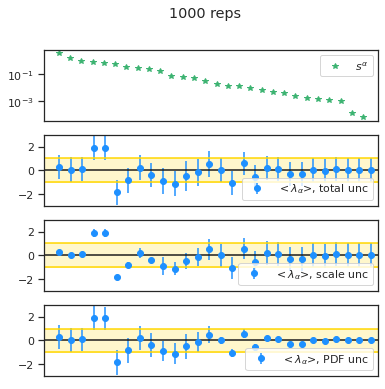
\includegraphics[width=0.6\columnwidth]{correlations/plots/lambdas1000.png}}
    \end{center}
  \vspace{-0.55cm}
  \caption{The $28$ positive eigenvalues, $s^\alpha$, of $S$ (top panel), shown in descending order, and 28 nuisance parameters $\lambda_\alpha$ corresponding to the $28$ eigenvectors $\beta_\alpha$ (lower three panels), as given by Eqn.~\ref{eq:lambdabarfxrep}.The uncertainties in the nuisance parameters are shown in total (square roots of the diagonal entries of Eqn.~\ref{eq:Zbardefgen}, and broken down into the contribution from scale uncertainties alone (square roots of the diagonal entries of Eqn.~\ref{eq:zdefmat2}  and from PDF uncertainties (square roots of the diagonal entries of Eqn.~\ref{eq:covlambdagen}). The horizontal yellow bands highlight the region between $\pm 1$.}
  \label{fig:nuisancediag}
\end{figure}
%%%%%%%%%%%%%%%%%%%%%%%%%%%%%%%%%%%%%%%%%%%%%%%%%%%%%%%%%%%%

Recall that the prior for the nuisance parameters was a unit Gaussian centred on zero (Eqn.~\ref{eq:priorf}). After fitting, we see that their variance remains close to one, showing that fitting to the data has not taught them a lot. Looking at the central values, those corresponding to the larger eigenvalues fluctuate about zero roughly in line with their uncertainties, but those for the smaller eigenvalues stay centred on zero. This shows us that it is only the eigenvectors corresponding to the largest $\sim$ 18 eigenvalues which are relevant in the PDF determination; the others are associated with such small theory uncertainty effects that the fit ignores them.

It helps to separate out the two contributions to the uncertainty on the nuisance parameters, namely:
\begin{enumerate}
\item the scale uncertainty (Eqn.~\ref{eq:zdefmat2});
\item the PDF uncertainty (Eqn.~\ref{eq:covlambdagen}).
\end{enumerate}
These are shown as the lower two panels in Fig.~\ref{fig:nuisancediag}. For fitting a single replica, the scale uncertainty in the nuisance parameters with the largest eigenvalues is reduced substantially, showing that the MHOU along these directions has been learnt in the fitting process, just as it was in the simple models in Secs.~\ref{sec:p1} and ~\ref{sec:p2}. However, this effect is almost entirely compensated by an additional uncertainty from fluctuations in the PDFs, so that overall there is almost no learning of the MHOUs. Consequently, the PDFs will contain very little information about the MHOUs, and so when making predictions using them the MHOUs will be almost entirely decorrelated with those in the prediction.
%%%%%%%%%%%%%%%%%%%%%%%%%%%%%%%%%%%%%%%%%%%%%%%%%%%%%%%%%%%%
  \begin{figure}[h!]
    \begin{center}
    \makebox{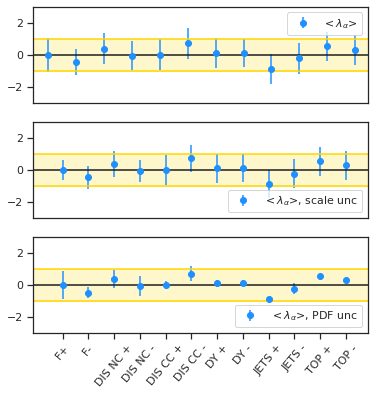
\includegraphics[width=0.6\columnwidth]{correlations/plots/lambdas_phys.png}}
    \end{center}
  \vspace{-0.55cm}
  \caption{Nuisance parameters $\lambda$ for directions in the space of scale variations corresponding to up/down changes in factorisation scale, and in renormalisation scale for the five types of processes in the determination of the $9$-pt theory covariance matrix for MHOUs. Uncertainties in the nuisance parameters are shown in total, and broken down into the contribution from scale uncertainties alone and from PDF uncertainties, just as in Fig.\ref{fig:nuisancediag}. The horizontal yellow bands highlight the region between $\pm 1$.}
  \label{fig:nuisancephys}
\end{figure}
%%%%%%%%%%%%%%%%%%%%%%%%%%%%%%%%%%%%%%%%%%%%%%%%%%%%%%%%%%%%
Having seen that some directions of MHOU are more relevant in the fit, we may wonder whether these have a physical interpretation; in Fig.~\ref{fig:evecs1} of Chapter \ref{chapter:mhous} that the largest eigenvectors of $S$ were driven by factorisation scale variation and then renormalisation scale variation for DIS NC. To investigate this, we can switch bases, choosing $\beta_\alpha$ to correspond to factorisation scale variations (up/down) and renormalisation scale variations (up/down for each process). Fig.~\ref{fig:nuisancephys} is a similar plot to Fig.~\ref{fig:nuisancediag}, but for this ``physical" basis. 

We see that the central values fluctuate about zero, but stayin the $\pm$1 band, showing again that the impact of fitting the data on the nuisance parameters is not large. This is reassuring as it backs up the choice of central scales and the choice of range of scale variations (the latter being implicit in the prior for $\lambda_\alpha$. Looking just at the scale uncertainty, it is apparent that the factorisation scale variation nuisance parameters have learnt the most information, which makes sense as factorisation scale variation is common to all data in the fit. NC DIS, being the largest process, is also learnt about to some extent. However, including the PDF uncertainty washes out these effects. In particular, the uncertainties in these directions can be slightly greater than one in total; in fact there is less learnt about the factorisation scale nuisance parameters that we had supposed in the prior.

We are starting to see that the decorrelation between MHOUs in the PDF fit and the predictions is likely to be large; it is very difficult to learn the MHOUs from the data. This is not only because of the fluctuations in the data and the universality of the PDFs, but also because of the functional uncertainty. This causes uncorrelated fluctuations of the PDFs which wash out the remaining correlations. 

Having said this, there are still shifts in the nuisance parameters, and these will lead to shifts in the theory prediction central values. In this way, information from the data in the fit can propagate into the predictions through the correlations in the theory uncertainties. 

\subsection{Autopredictions}
As described in Sec.~\ref{sec:p1}, autopredictions are where we fit a PDF and then use that PDF to make predictions for the data that went into the PDF. These are essentially postdictions, and are ideal for testing the extent of decorrelation between theory uncertainties in the PDF fit and in the (auto)predictions. 
%%%%%%%%%%%%%%%%%%%%%%%%%%%%%%%%%%%%%%%%%%%%%%%%%%%%%%%%%%%%%%%%%%
\begin{figure}[H]
    \begin{center}
    \makebox{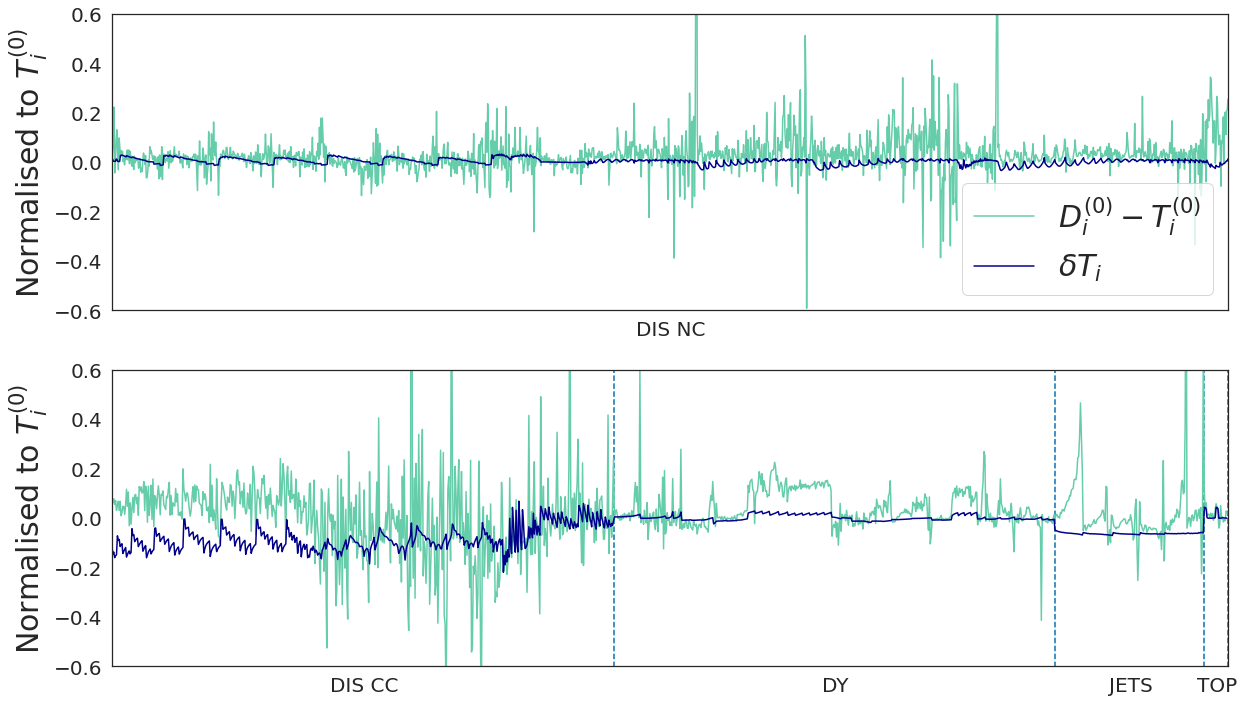
\includegraphics[width=0.99\columnwidth]{correlations/plots/autopredictions_9_1000.png}}
    \end{center}
  \vspace{-0.55cm}
  \caption{The shifts $\delta T_i$, Eqn.~\ref{eq:shiftmult}, compared to the differences between theory and data, $D_i-T^{(0)}_i$, both normalised to $T^{(0)}_i$.} 
  \label{fig:shifts}
\end{figure}
%%%%%%%%%%%%%%%%%%%%%%%%%%%%%%%%%%%%%%%%%%%%%%%%%%%%%%%%%%%%%%%%%%
Although this situation is somewhat artificial because experiments are never redone in exactly the same way, the implications of this investigation will be general. This is because for a global fit of this size (2819 data points, 35 datasets and 5 processes), removing only one of the smaller datasets has negligible impact on the PDFs. Removing even a large dataset will only increase PDF uncertainties without affecting the theory uncertainties for the remaining data. This means that if we did the fit with a certain dataset removed, and did the analysis with that fit instead, we would instead have a genuine prediction, and the correlations between MHOUs in the PDF and the prediction would be very close to what we have for the autopredictions.
%%%%%%%%%%%%%%%%%%%%%%%%%%%%%%%%%%%%%%%%%%%%%%%%%%%%%%%%%%%%%%%%%%
\begin{figure}[h]
    \begin{center}
    \makebox{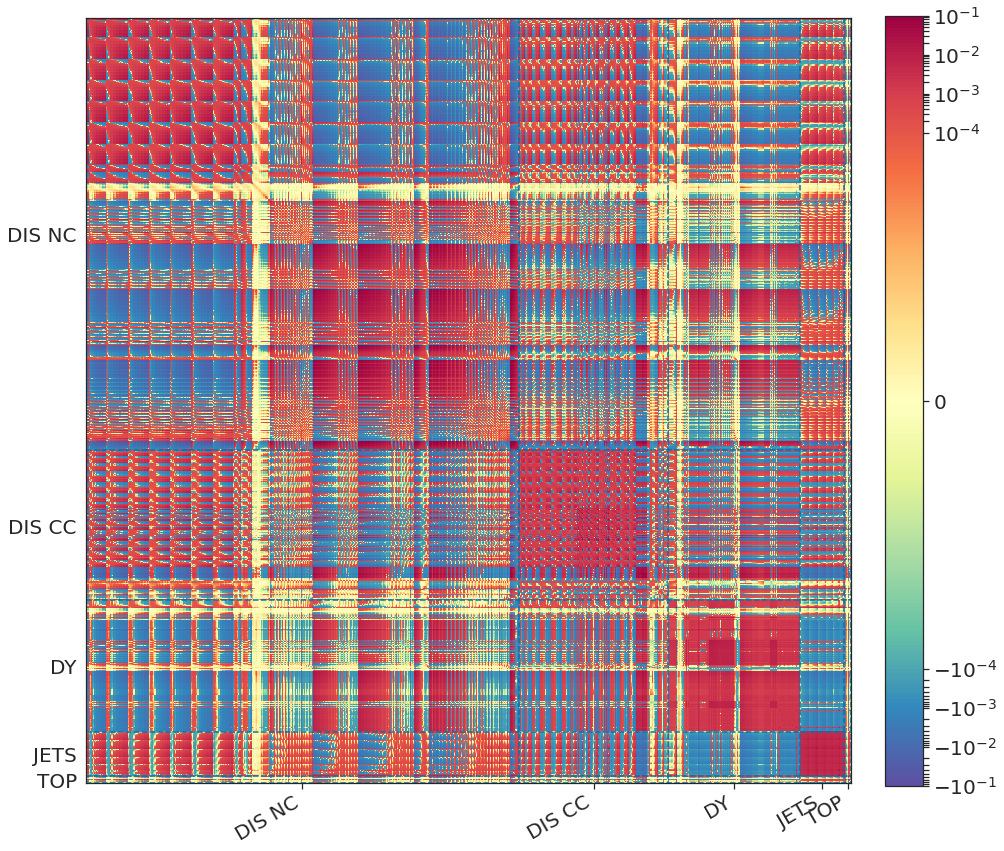
\includegraphics[width=0.45\columnwidth]{correlations/plots/P_covmat_cutscale.png}}
    \makebox{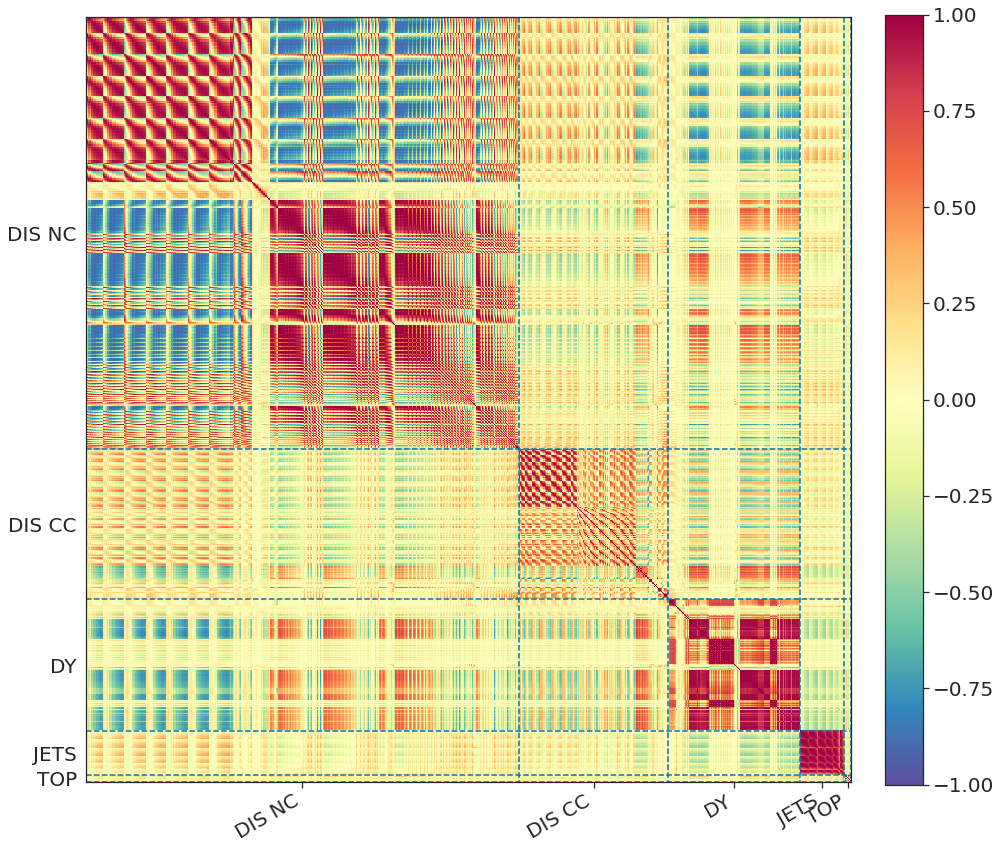
\includegraphics[width=0.45\columnwidth]{correlations/plots/pcorrmat.png}}  
  \end{center}
  \vspace{-0.55cm}
  \caption{The autoprediction covariance matrix $P_{ij}$ Eqn.~\ref{eq:covTfitfun}, normalised to the theoretical predictions $T^{(0)}_i$ (left), and the corresponding corrrelation matrix $P_{ij}/\sqrt{P_{ii}P_{jj}}$ (right).}
  \label{fig:P}
\end{figure}
%%%%%%%%%%%%%%%%%%%%%%%%%%%%%%%%%%%%%%%%%%%%%%%%%%%%%%%%%%%%%%%%%%
%%%%%%%%%%%%%%%%%%%%%%%%%%%%%%%%%%%%%%%%%%%%%%%%%%%%%%%%%%%%%%%%%%
 \begin{figure}[h]
    \begin{center}
    \makebox{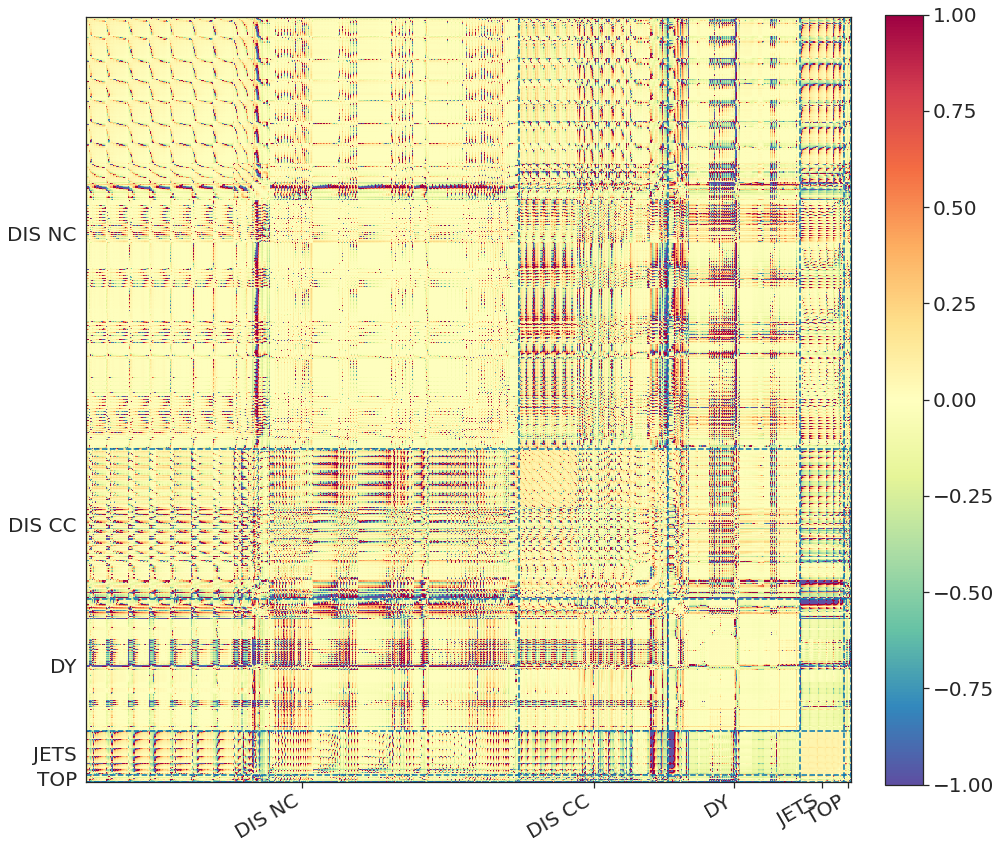
\includegraphics[width=0.45\columnwidth]{correlations/plots/AP.png}}
     \makebox{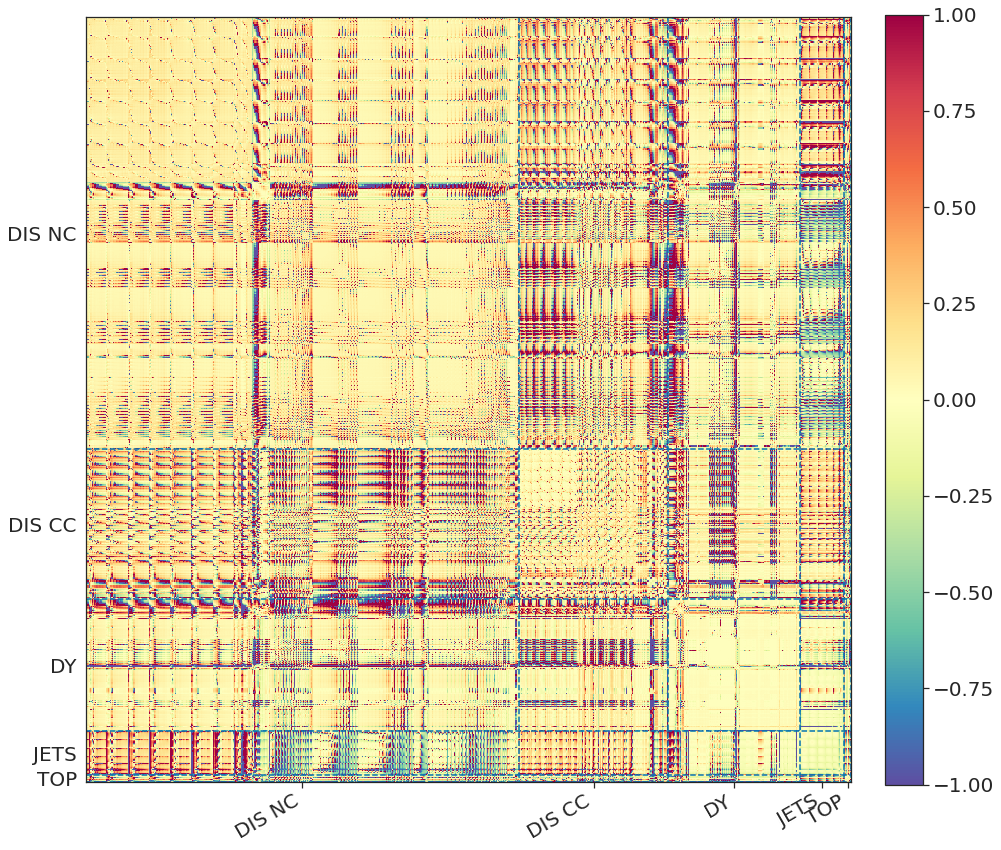
\includegraphics[width=0.45\columnwidth]{correlations/plots/PconP.png}}
   \end{center}
  \vspace{-0.55cm}
  \caption{The difference $(P^{\rm sim}_{ij}-P_{ij})/P_{ij}$ , with $P^{\rm sim}_{ij}$ computed using Eqn.~\ref{eq:covTfitfunapprox} (left), and the difference $(P^{\rm con}_{ij}-P_{ij})/P_{ij}$, where $P^{\rm con}_{ij}=X_{ij}+S_{ij}$ (right).}
 \label{fig:PminA}
\end{figure}
%%%%%%%%%%%%%%%%%%%%%%%%%%%%%%%%%%%%%%%%%%%%%%%%%%%%%%%%%%%%%%%%%%

To make the correlated autopredictions, we first compute $\delta T_i$ (Eqn.~\ref{eq:shiftmult}). This is the shift in theory predictions arising due to theory correlations. We show this in Fig.~\ref{fig:shifts}, normalised to the orginal theoretical prediction $T^{(0)}_i$. We also show $D_i^{(0)}-T_i^{(0)}$ for comparison. The shifts tend to be small and so they can be ignored. However, for some datasets (especially CHORUS and inclusive jets) there is a systematic overall shift of order $D_i^{(0)}-T_i^{(0)}$.

For the change in uncertainties, we examine $P$ (Eqn.~\ref{eq:covTfitfun}), shown as a heatmap alongside its correlation matrix in Fig.~\ref{fig:P}. $P$ includes the PDF uncertainties (from uncertainties in the input data and theory), the theory uncertainties in the autoprediction, and the correlation. Unsurprisingly, there are very large correlations in the autopredictions within datasets, especially for nearby kinematic regions. However, there are also significant effects between datasets. These come from experimental uncertainty correlations and also theory uncertainty correlations and correlations due to the smooth PDFs which underlie all the data.

We saw that in general $Y_{ii} < X_{ii}$, suggesting that $P_{sim}$ (Eqn.~\ref{eq:covTfitfunapprox}) could be an appropriate description of $P$. In Fig.~\ref{fig:PminA} we show the difference between $P$ and $P_{sim}$, and shows that in general the difference is small so the simplification works quite well. 
%%%%%%%%%%%%%%%%%%%%%%%%%%%%%%%%%%%%%%%%%%%%%%%%%%%%%%%%%%%%%%%%%%
 \begin{figure}[H]
    \begin{center}
    \makebox{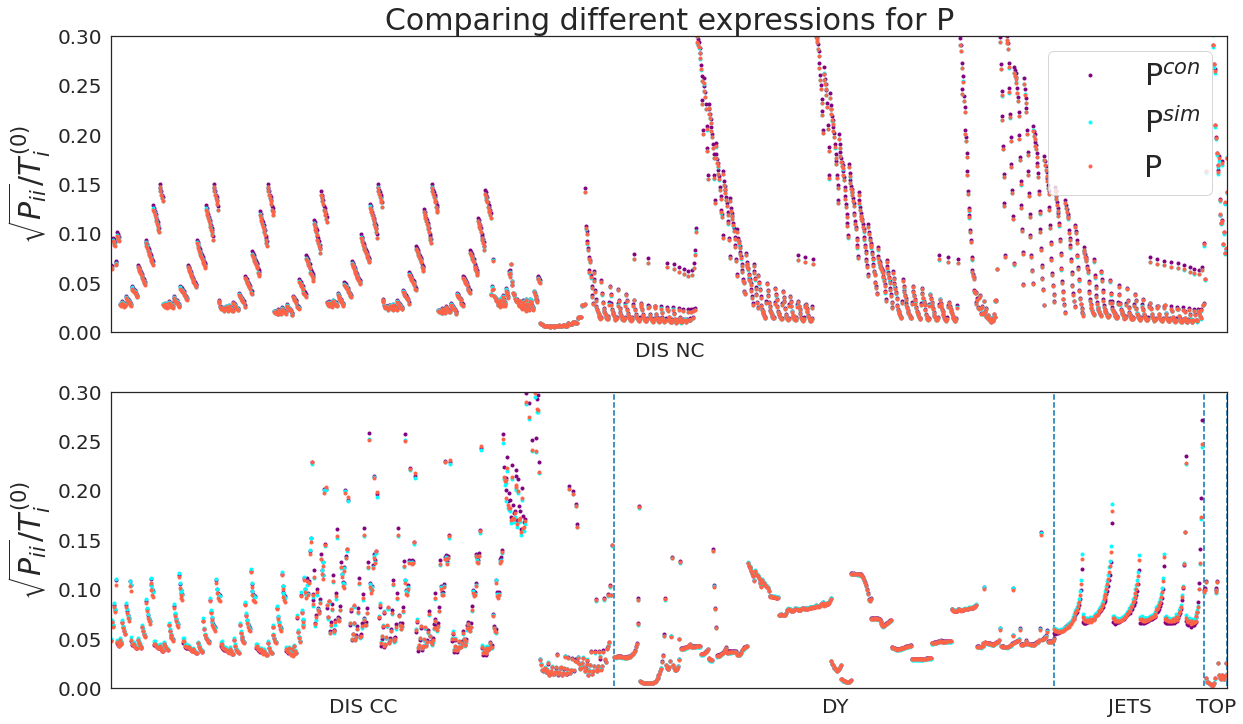
\includegraphics[width=0.99\columnwidth]{correlations/plots/pcomparison1000nopos.png}}
    \end{center}
  \vspace{-0.55cm}
  \caption{The percentage uncertainties of the autoprediction $\sqrt{P_{ii}}/T^{(0)}_i$. The simplified result $\sqrt{P^{\rm sim}_{ii}}/T^{(0)}_i$, and the conservative result, $\sqrt{P^{\rm con}_{ii}}/T^{(0)}_i$ are also shown.}
  \label{fig:Pdiag}
\end{figure}
%%%%%%%%%%%%%%%%%%%%%%%%%%%%%%%%%%%%%%%%%%%%%%%%%%%%%%%%%%%%%%%%%%
%%%%%%%%%%%%%%%%%%%%%%%%%%%%%%%%%%%%%%%%%%%%%%%%%%%%%%%%%%%%%%%%%%
 \begin{figure}[H]
    \begin{center}
    \makebox{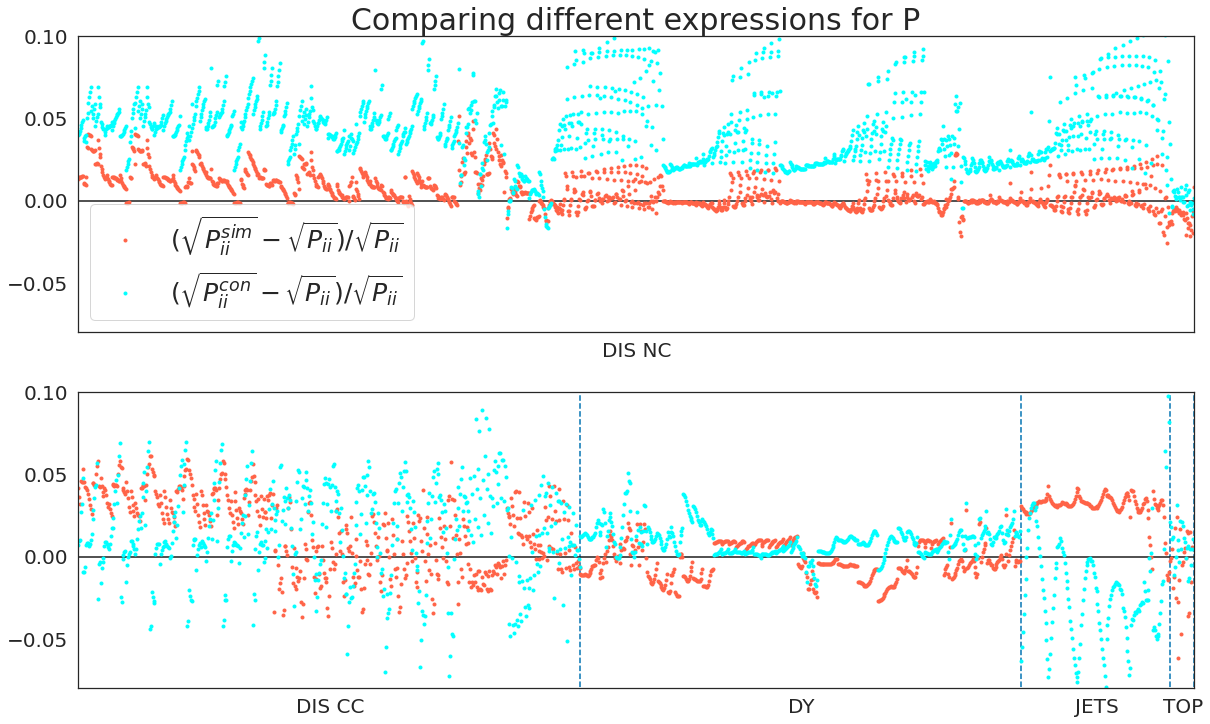
\includegraphics[width=0.99\columnwidth]{correlations/plots/pdiag1000nopos.png}}
    \end{center}
  \vspace{-0.55cm}
  \caption{The diagonal differences $\sqrt{P^{\rm sim}_{ii}}-\sqrt{P_{ii}}/\sqrt{P_{ii}}$, and $\sqrt{P^{\rm con}_{ii}}-\sqrt{P_{ii}}/\sqrt{P_{ii}}$. }
  \label{fig:Pdiagapprox}
\end{figure}
%%%%%%%%%%%%%%%%%%%%%%%%%%%%%%%%%%%%%%%%%%%%%%%%%%%%%%%%%%%%%%%%%%
Likewise, we have previously argued that the conservative prescription, where the theory uncertainty in the PDF and the prediction are uncorrelated, should be reasonable, because the level of correlation is likely to be small. Here we simply add the PDF uncertainty and the prediction uncertainty in quadrature, i.e. $P_{con} = X + S$. We are now in a position to test the validity of this claim. Fig.~\ref{fig:PminA} also shows the difference between $P$ and $P_{con}$. The approximation is not as good as $P_{sim}$, as expected, but it is still fairly accurate for most data points.

Taking a closer look at the uncertainties, we can look at the \% per-point uncertainties, shown in Fig.~\ref{fig:Pdiag}. We show all three versions of $P$, i.e. $\sqrt{P_{ii}}$, $\sqrt{P^{\rm sim}_{ii}}$ and $\sqrt{P^{\rm con}_{ii}}$. They are very similar and hard to distinguish, so we also show in 
Fig.~\ref{fig:Pdiagapprox} the \% difference in the uncertainties. From this we see that the conservative approach overestimates the uncertainty by at most $\sim$10\%, and usually much less (not 100\%, as suggested in Ref.~\cite{Harland-Lang:2018bxd}). The simplification (Eqn.~\ref{eq:covTfitfunapprox}) deviates by at most $\sim$5\%. Note that these results must be evaluated in the context of the overall reliability of the MHOUs, which here were estimated by scale variation, and therefore the reliability of the choice of prescription which was used to construct $S$.

%%%%%%%%%%%%%%%%%%%%%%%%%%%%%%%%%%%%%%%%%%%%%%%%%%%%%%%%%%%%%%%%%%
\begin{figure}[h]
    \begin{center}
    \makebox{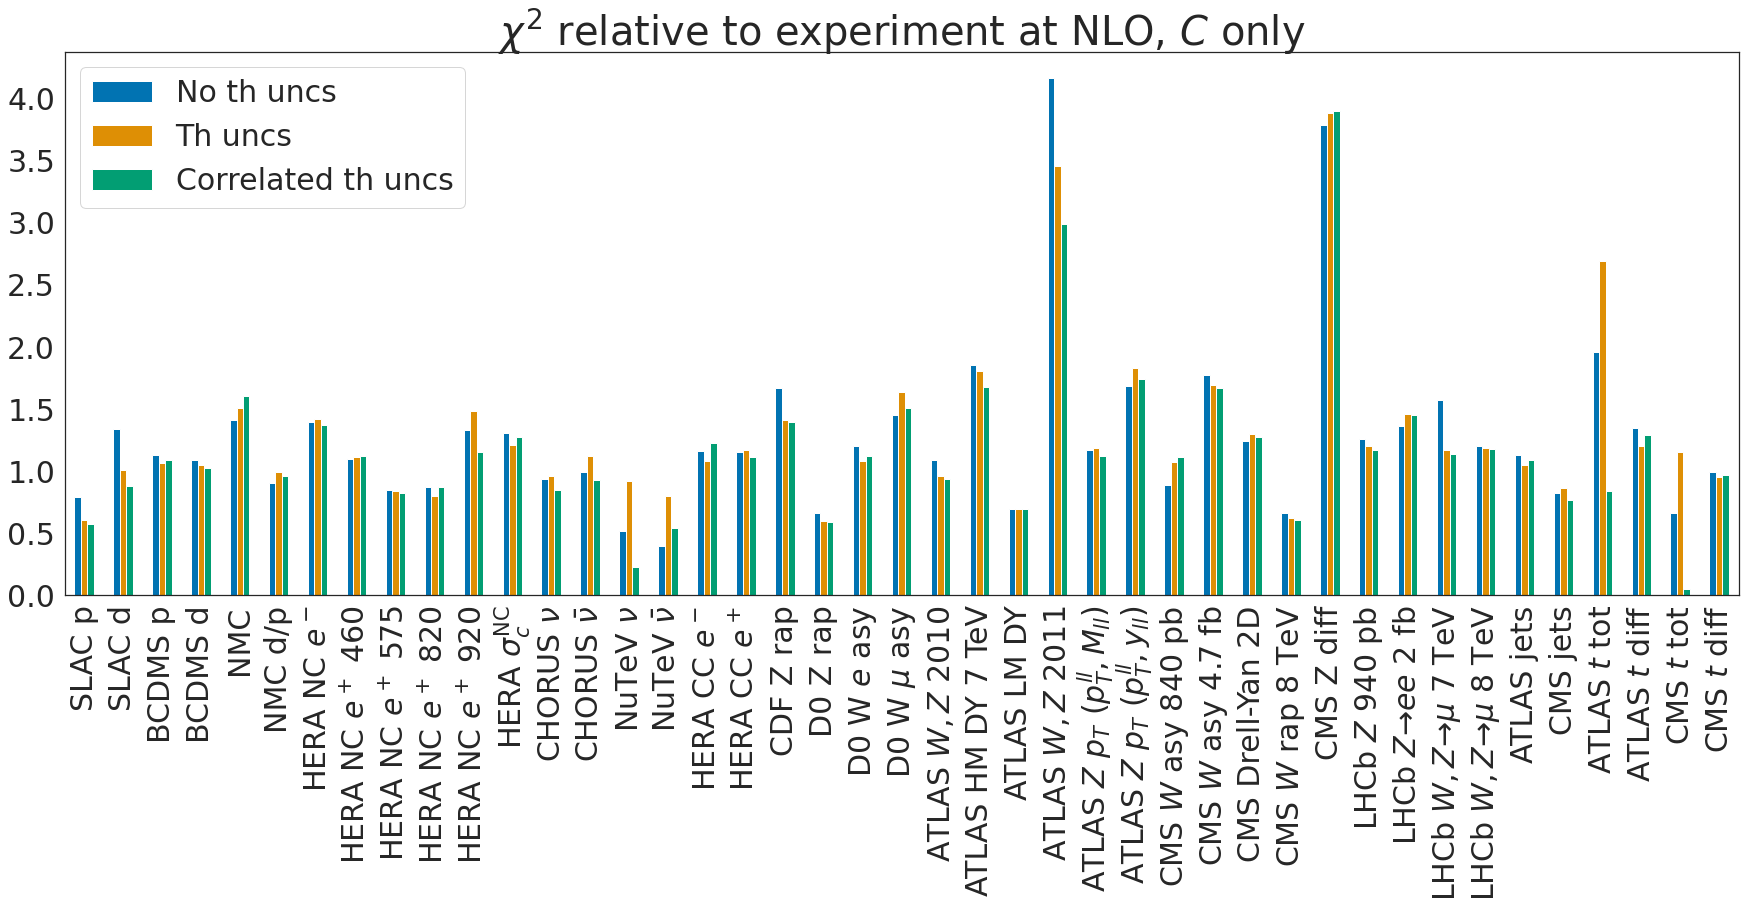
\includegraphics[width=0.99\columnwidth]{correlations/plots/chi2_auto.png}}
    \end{center}
  \vspace{-0.55cm}
  \caption{The experimental $\chi^2$ to each data set, comparing the original result of the NLO fit with no theory uncertainties to the fit with theory uncertainties, and then including the correlated shift in the autopredictions.}
  \label{fig:chi2auto}
\end{figure}
%%%%%%%%%%%%%%%%%%%%%%%%%%%%%%%%%%%%%%%%%%%%%%%%%%%%%%%%%%%%%%%%%%
%%%%%%%%%%%%%%%%%%%%%%%%%%%%%%%%%%%%%%%%%%%%%%%%%%%%%%%%%%%%%%%%%%
\begin{table}[H]
\centering
\begin{tabular}{|l||lllll|l|}
\hline
                   & \textbf{DIS NC} & \textbf{DIS CC} & \textbf{DY} & \textbf{JETS} & \textbf{TOP} & \textbf{Total} \\
                   \hline
No th uncs         & 1.13            & 0.98            & 1.56        & 0.88         & 1.20         & 1.17           \\
Uncorr th uncs     & 1.15            & 1.06            & 1.53        & 0.90         & 1.27         & 1.19           \\
Correlated th uncs & 1.09            & 0.91           & 1.47        & 0.83         & 0.97        & 1.10    \\
\hline
\end{tabular}
%%%%%%%%%%%%%%%%%%%%%%%%%%%%%%%%%%%%%%%%%%%%%%%%%%%%%%%%%%%%%%%%%%
\caption{The experimental $\chi^2$ per data point for each process, comparing the original result of the NLO fit with no theory uncertainties to the fit with theory uncertainties, and then including the correlated shift in the autopredictions.}
  \label{tab:chisq}
\end{table}
Keeping this, and the fact that these are autopredictions, in mind, it's interesting to see whether the shifts improve the autopredictions. In Fig.~\ref{fig:chi2auto} we show the $\chi^2$ of the autopredictions, using the experimental covariance matrix only, for the following autoprediction central values:
\begin{itemize}
\item No theory uncertainty;
\item Theory uncertainty in the fit;
\item Theory uncertainty in the fit, and correlated shift included.
\end{itemize}
We use only the experimental covariance matrix, in order to isolate the effects due to the changing central value from those due to adding additional uncertainties. 

The results for all cases are very similar. Including the theory uncertainty in the fit has mixed results; some predictions get better at the expense of others getting worse. This is because the main effect of including theory uncertainties is to rebalance the fit. When the correlated shift is also included, the fit to most datasets improves, in some cases substantially. The exact values are broken down by process in Tab.~\ref{tab:chisq}. When including theory uncertainties, the $\chi^2$ goes up slightly from 1.17 to 1.19. However, when the correlated shift is added, there is a significant improvement across all processes, with the total $\chi^2$ dropping to 1.10.

\subsection{Predictions for an existing process: top production}
Finally we can consider genuine predictions for experiments that weren't used in the PDF fits. These can either be for processes already in the fit, or for new ones. Here we consider the former, and in the next subsection we'll end with the latter.

We look at $t\bar{t}$ production rapidity distributions in two channels (dilepton and lepton + jets), measured by CMS at 13 TeV~\cite{Sirunyan:2018ucr,Sirunyan:2018wem}. There are a couple of reasons for this choice:
\begin{itemize}
\item The base fit contains $t\bar{t}$ total cross sections at 7, 8 and 13 TeV and normalised rapidity distributions at 8 TeV, all from both ATLAS and CMS.
\item The NLO theory uncertainty for the 13 TeV data is $\sim$10\%, considerably larger than the PDF uncertainty.
\end{itemize}
Both these things mean that we'd expect the correlation between the theory uncertainties in these data and the 13 TeV distributions to be high, and so we should see some of the largest effects currently possible with these PDFs. The CMS 13 TeV $t\bar{t}$ rapidity predictions were computed using the same procedure as the 8 TeV distributions in Ref.~\cite{Ball:2017nwa}:NLO theoretical predictions were been generated with {\tt Sherpa}~\cite{Gleisberg:2008ta}, in a format compliant with {\tt APPLgrid}~\cite{Carli:2010rw}, using the {\tt MCgrid} 
code~\cite{DelDebbio:2013kxa} and the {\tt Rivet}~\cite{Buckley:2010ar} analysis package, with {\tt OpenLoops}~\cite{Cascioli:2011va} for the NLO 
matrix elements. Renormalization and factorization scales have been chosen based on the recommendation of 
Ref.~\cite{Czakon:2016dgf} as $H_T/4$.

Our aim is to calculate $\Ptil$ and $\delta \Ttil$, so we first need to calculate $\Stil$ (the theory covariance matrix for the predictions) and $\Shat$ (the theory correlations between the predictions and the theories in the fit). Then we need to find $\Xtil$ and $\Xhat$ (the PDF uncertainties) and $\Yhat$ (the correlations of the data in the fit with the new predictions). If we're just going to find $\Ptil_{sim}$ rather than $\Ptil$, we won't need $\Yhat$, and therefore won't need the data replicas. Further, if we're going to use $\Ptil_{cons}$, we only need $\Xtil$ and $\Stil$, and therefore won't need any information about the replicas in the fit. These variations are therefore significantly simpler calculations.
%%%%%%%%%%%%%%%%%%%%%%%%%%%%%%%%%%%%%%%%%%%%%%%%%%%%%%%%%%%%%%%%%%
\begin{figure}[t!]
    \begin{center}
    \makebox{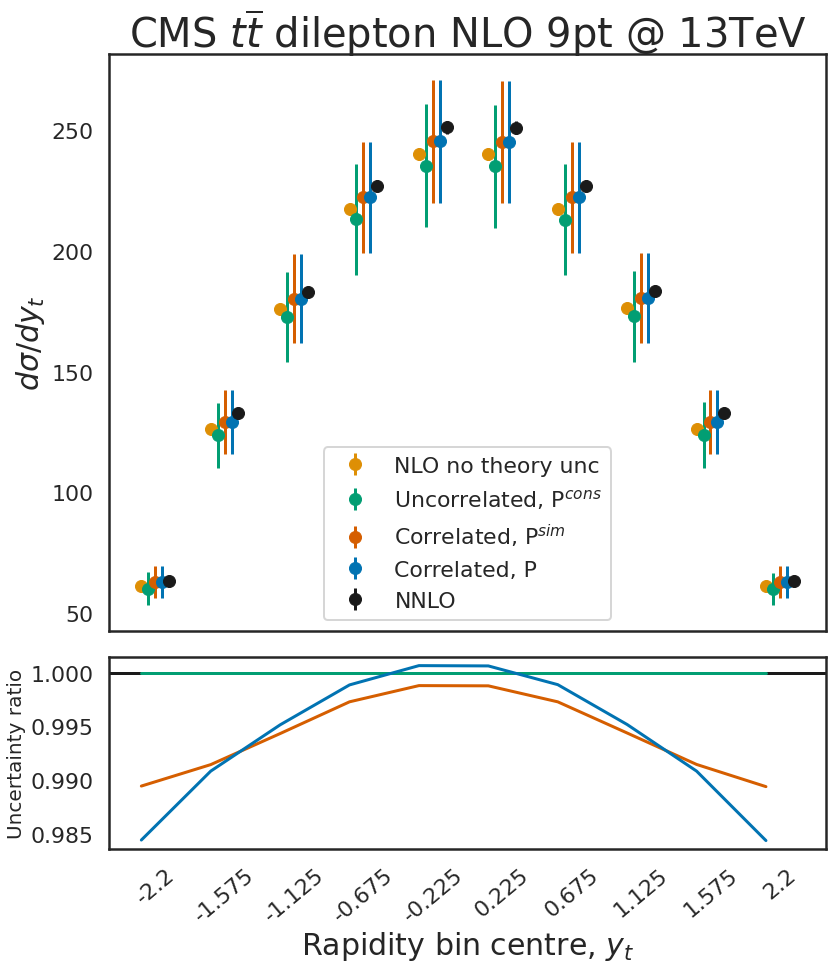
\includegraphics[width=0.45\columnwidth]{correlations/plots/cmstopcombined_ll.png}}
   \makebox{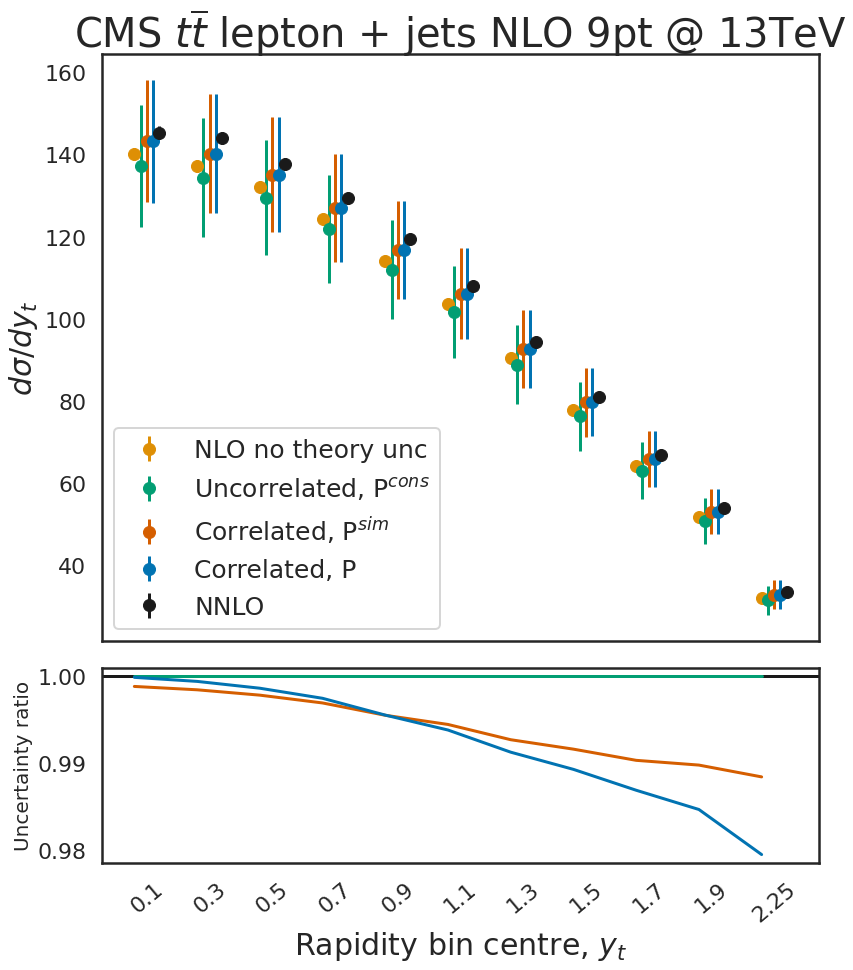
\includegraphics[width=0.46\columnwidth]{correlations/plots/cmstopcombined_lj.png}}
    \end{center}
  \vspace{-0.55cm}
  \caption{The upper two panels show predictions for $t\bar{t}$ unnormalised rapidity distribution data taken at 13TeV by CMS, the dilepton rapidity distribution \cite{Sirunyan:2018ucr} (left) and the lepton+jets distribution \cite{Sirunyan:2018wem} (right). The four predictions show: the NLO fit with no MHOUs, PDF error only; the combined PDF and MHOU fit, ignoring correlations (thus $\sqrt{P_{II}^{\rm con}}$); the correlated result including the shift, and uncertainty computed using the simplified result (thus $\sqrt{P_{II}^{\rm sim}}$); the result with the same shift, but with the correlations included exactly (thus $P_{II}$), and the NNLO result with no MHOU. In the lower two panels we show the uncertainties in the same distributions, but normalised to the conservative result (thus $\sqrt{P_{II}^{\rm sim}/P_{II}^{\rm con}}$ and $\sqrt{P_{II}/P_{II}^{\rm con}}$).}
  \label{fig:CMSttbar}
\end{figure}
%%%%%%%%%%%%%%%%%%%%%%%%%%%%%%%%%%%%%%%%%%%%%%%%%%%%%%%%%%%%%%%%%%

The predictions are shown in Fig.~\ref{fig:CMSttbar}. The correlated shift is sizeable, about 5\%, but this is still comfortably within the $\sim$10\% theory uncertainty. We'd anticipate this given that Fig.~\ref{fig:nuisancephys} tells us that the shift in nuisance parameters for the top renormalisation scale variation is also well within uncertainties. We also see that the shift is almost fully correlated across the whole distribution. This is because these are unnormalised distributions, so there is the restriction that they must sum to the total cross section. They are therefore strongly correlated with the measurements of the total cross section in the fit. We can confirm this by breaking down the contributions to the shift from the different fitted data points, seen in Table ~\ref{tab:deltilcons}. The six total cross section measurements are responsibile for the vast majority of the shift, with the 8 TeV normalised rapidity distributions pushing the shift back down by about 25\%. The rest of the data have almost no impact.
%%%%%%%%%%%%%%%%%%%%%%%%%%%%%%%%%%%%%%%%%%%%%%%%%%%%%%%%%%%%%%%%%%
\begin{table}[h]
  \centering
  \scriptsize
  \renewcommand{\arraystretch}{1.4}
  \begin{tabular}{|llll|llll|l|}
   \hline
 {\bf ATLAS} &&&& {\bf CMS} &&&& {\bf Other}\\
 {\it tot} &&&{\it diff} &{\it tot}&&&{\it diff} & \\
  7 TeV &  8 TeV & 13 TeV & 8 TeV &7 TeV & 8 TeV &13 TeV & 8 TeV & \\
    \hline
 0.37 & 0.11 & 0.24 & -0.21 & 0.26 & 0.21 & 0.07 & -0.04 & -0.01 \\
\hline
  \end{tabular}
\caption{The fractional contributions of different data sets included in the fit to the
shifts in the top rapidity distributions, averaged over all 21 data points.}
\label{tab:deltilcons}
\end{table}
%%%%%%%%%%%%%%%%%%%%%%%%%%%%%%%%%%%%%%%%%%%%%%%%%%%%%%%%%%%%%%%%%%

To see if the shift improves the predictions, we can compare it to the known NNLO-NLO shift, just like we did in Chapter ~\ref{chapter:mhous}. Therefore, in Fig.~\ref{fig:CMSttbar} we also show the full NNLO result (without theory uncertainties). It's interesting that the shift due to correlations, which we saw is driven by the $t\bar{t}$ total cross section data, largely accounts for the NNLO correction; the data know that the NLO theory predictions are a bit low, and that knowledge is propagated into the predictions for the 13 TeV rapidity distributions. 
%%%%%%%%%%%%%%%%%%%%%%%%%%%%%%%%%%%%%%%%%%%%%%%%%%%%%%%%%%%%%%%%%% 
\begin{table}[h]
\centering
\begin{tabular}{|l||lll|}
\hline
                   & \textbf{dilepton} & \textbf{lepton+jet} & \textbf{combined} \\
                   \hline
No th uncs         &    0.55         &    0.37         & 0.46             \\
Uncorr th uncs     &   0.57         &    0.42         & 0.49               \\
Correlated th uncs &     0.49        &   0.37        & 0.43         \\
NNLO, no th uncs &    0.45        &    0.39     & 0.42          \\
\hline
\end{tabular}
\caption{The experimental $\chi^2$ per data point for the CMS 13 TeV top dilepton and lepton+jet rapidity distributions, comparing the original result of the NLO fit with no theory uncertainties to the fit with theory uncertainties, and then including the correlated shift in the autopredictions. Also shown for comparison is the result in a NNLO fit with no theory uncertainties.}
  \label{tab:topchisq}
\end{table}
%%%%%%%%%%%%%%%%%%%%%%%%%%%%%%%%%%%%%%%%%%%%%%%%%%%%%%%%%%%%%%%%%%
Table ~\ref{tab:topchisq} compares the $\chi^2$s for these data (using $C$ only, as before). On including theory uncertainties the $\chi^2$ goes up, presumably because these data are deweighted in the fit. But then adding the correlated shift leads to a significant improvement, down to the level of the NNLO calculations. 

These improvements demonstrate the power of the shifts, and their potential as a new method whereby theory correlations can enable us to use experimental data to improve theory predictions. We note that this method will have maximum efficacy when we already have a lot of experimental data for that process in the fit, as is the case here.

We now look at the change in uncertainties. Given that this change is too small to evaluate by eye, in Fig.~\ref{fig:CMSttbar} we include a lower panel showing the uncertainties as ratios to the conservative prescription. We confirm that there is almost full decorrelation, noting that the exact calculation gives results less than 2\% below the conservative (uncorrelated) result. The simplified calculation gives results very close to exact across the entire kinematic range. Note that while $P_{II}^{sim} < P_{II}^{con}$ for all values, $P_{II}$ sneaks in slightly higher for a couple of bins, as we saw is possible in Fig.~\ref{fig:plot3}.
%%%%%%%%%%%%%%%%%%%%%%%%%%%%%%%%%%%%%%%%%%%%%%%%%%%%%%%%%%%%%%%%%%
\begin{figure}[t]
    \begin{center}
    \makebox{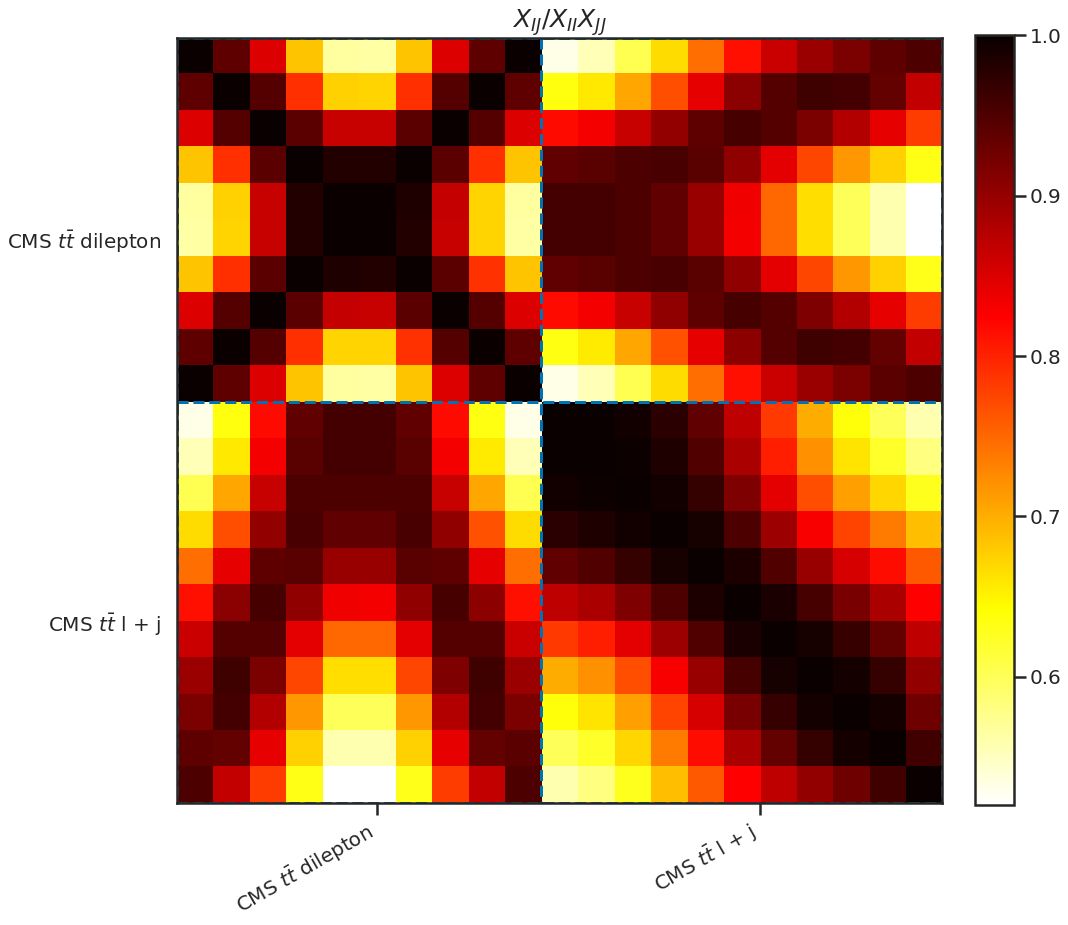
\includegraphics[width=0.49\columnwidth]{correlations/plots/Xcorrln.png}}
   \makebox{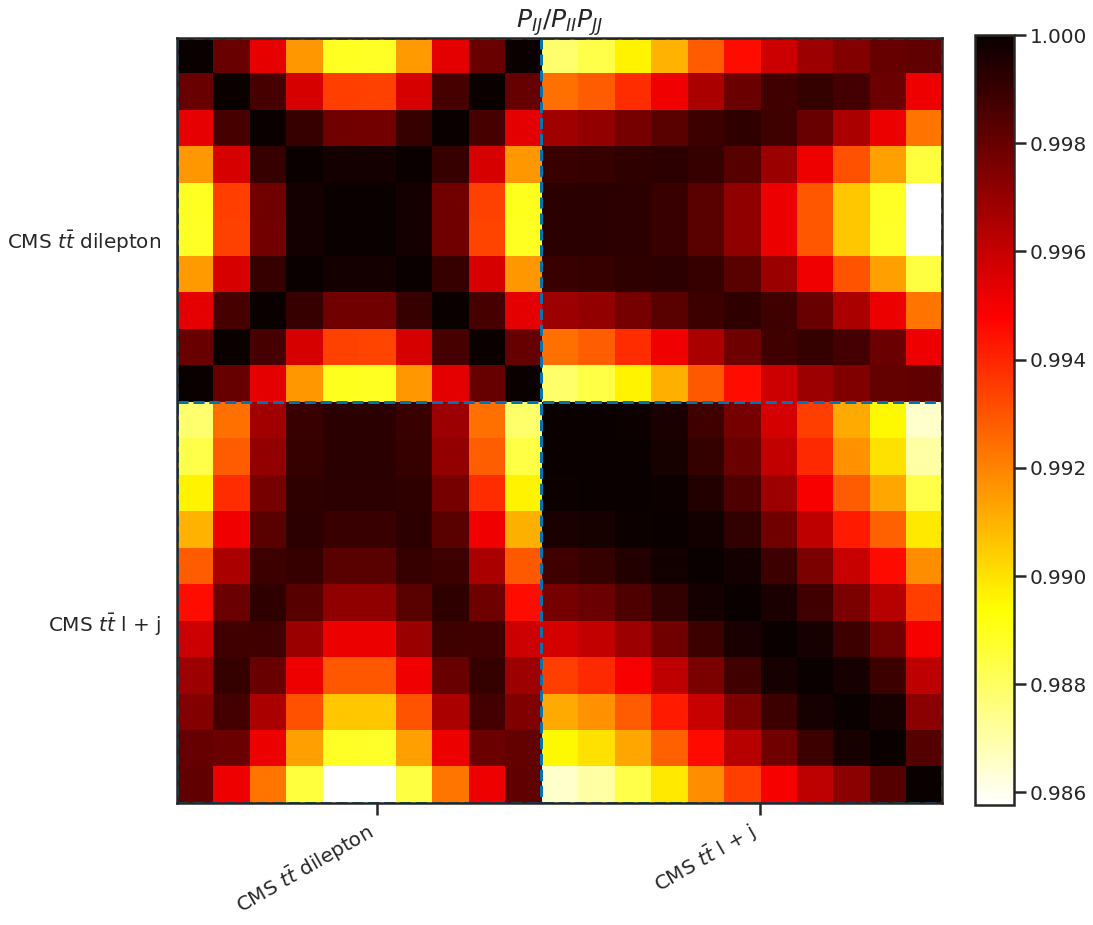
\includegraphics[width=0.49\columnwidth]{correlations/plots/Pcorrln2.png}}
    \end{center}
  \vspace{-0.55cm}
  \caption{The left hand plot shows the correlation matrix $\Xtil_{IJ}/\sqrt{\Xtil_{II}\Xtil_{JJ}}$ of the contribution of the PDF uncertainties to the predictions for the 13 TeV rapidity distributions by CMS: the right hand plot shows the correlation matrix $\Ptil_{IJ}/\sqrt{\Ptil_{II}\Ptil_{JJ}}$ of the total uncertainties including the correlated theoretical uncertainties. Note the expanded scales on these plots.} 
  \label{fig:CMSttbarcorrlns}
\end{figure}
%%%%%%%%%%%%%%%%%%%%%%%%%%%%%%%%%%%%%%%%%%%%%%%%%%%%%%%%%%%%%%%%%%

The theory uncertainties in the predictions are all highly correlated with one another, including between the two rapidity distributions. We can see this by looking at the correlation matrices for $\Xtil$ and $\Ptil$, shown in 
Fig.~\ref{fig:CMSttbarcorrlns}. The predictions are all to start with more than 60\% correlated by the PDF. Then, when correlated theory uncertainties are included, the correlations bump up to $>$ 98\%. We saw before that this is due to the constraint that they must all sum to give the total cross section. The pattern of correlations nicely shows the symmetry within the dilepton distribution, and with the lepton + jets distribution; the greater the rapidity separation, the smaller the correlation.

\subsection{Predicting a new process: Higgs production}
At last we can make some predictions for a new process: one outwith the fit. For this we choose Higgs production via gluon fusion. We calculate the total cross section at 14 TeV using {\tt  ggHiggs}~\cite{Ball:2013bra,Bonvini:2014jma,Bonvini:2016frm}.
Renormalization and factorization scales are set to half the Higgs' mass, and the computation is performed using rescaled effective theory.
%%%%%%%%%%%%%%%%%%%%%%%%%%%%%%%%%%%%%%%%%%%%%%%%%%%%%%%%%%%%%%%%%%
\begin{figure}[h!]
    \begin{center}
    \makebox{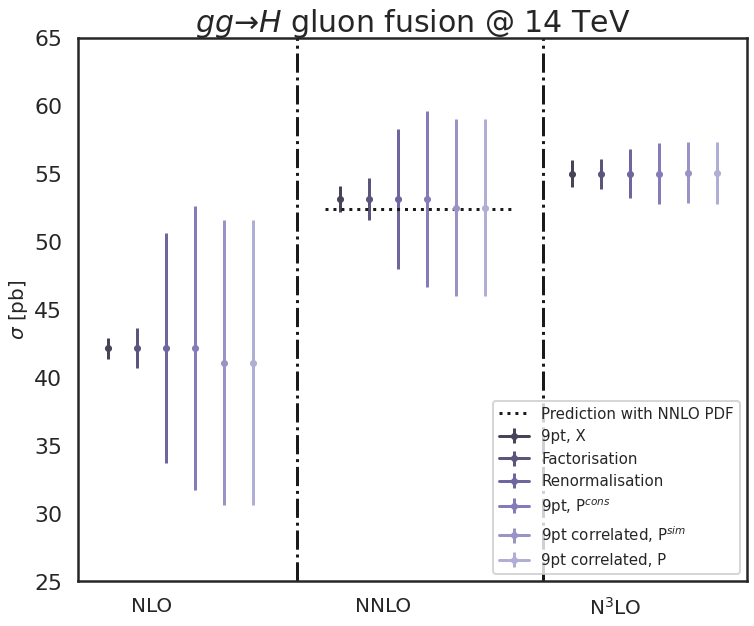
\includegraphics[width=0.9\columnwidth]{correlations/plots/higgs_plot_1000.png}}
    \end{center}
  \vspace{-0.55cm}
  \caption{Predictions for the Higgs total cross-section at 14 TeV, made using a variety of approximations. All results use NLO PDFs, while the Higgs total cross-section is computed at NLO (left panel), NNLO (centre panel) and N3LO (right panel). In each panel, we then have, from left to right: PDFs and cross-section both computed with No MHOU; MHOU included only in the PDF determination in the 9pt scheme; the same but with the factorization scale uncertainty (MHOU in PDF evolution) included; the same but with instead the renormalization scale uncertainty (MHOU in the Higgs cross-section); the total in the Higgs cross-section combined in quadrature, as recommended in Ref.~\cite{AbdulKhalek:2019ihb}; the total PDF plus 9pt MHOU, but now including also the correlation between theoretical uncertainties, using the approximate result; the same, but now using the exact result. In the centre panel we also show the NNLO prediction with NNLO PDFs (but no theoretical uncertainties), as a dashed line. }
  \label{fig:Higgs}
\end{figure}
%%%%%%%%%%%%%%%%%%%%%%%%%%%%%%%%%%%%%%%%%%%%%%%%%%%%%%%%%%%%%%%%%%

Our results are shown in in Fig.~\ref{fig:Higgs}. All results use the baseline NLO PDFs with MHOUs, but the parton-level Higgs cross sections are computed at NLO, NNLO and N$^3$LO. We break down the uncertainties into: 
\begin{enumerate}
\item The PDF uncertainty, $\Xtil$;
\item 3-point factorisation scale uncertainty; 
\item 3-point renormalisation scale uncertainty;
\item Conservative prescription, $\Ptil_{cons}$;
\item Simplified correlated, $\Ptil_{sim}$;
\item Fully correlated, $\Ptil$.
\end{enumerate}
Note that 2. and 3. sum to give the 5-point prescription in Chapter \ref{chapter:mhous}. 

At NLO the MHOU in the Higgs cross section (estimated by varying the Higgs renormalisation scale) completely dominates the other uncertainties, so the effect of correlations between the sources of MHOU is negligible.  At higher orders, the renormalisation scale uncertainty shrinks dramatically until it is comparable to the other sources of uncertainty at N$^3$LO. Notice also that the shift due to correlations is always very small compared to the overall uncertainty, and gets smaller order by order. Here, unlike for top production, the fit includes no information on Higgs production, so the renormalisation scale is totally uncorrelated. This means any information from the fit must propagate through factorisation scale uncertainties. We can see that at NNLO the small shit due to this pulls the NNLO prediction very close to the calculation using NNLO PDFs, although this is most likely coincidental. The effect of correlations on the total uncertainties is also minimal, and the difference between the simlified and full calculations is negligible. 

Note that if we used NNLO (or higher order) PDFs with MHOUs here (we can't - they don't exist!), the MHOU in the PDFs would have been smaller, and therefore the effects due to theory uncertainty correlations would be again smaller.

\section{Summary}
\label{sec:p5}

We considered the scenario where PDFs with theory uncertainties are used to make predictions with theory uncertainties. We studied the correlations between these two sources of theory uncertainties. We did this by recasting the theory uncertainties as nuisance parameters for each PDF replica, which contain information about the experimental data's impact on the theory uncertainties. We built our way through increasingly complex and correspondingly realistic models of the fitting procedure, isolating three distrinct decorrelation effects, namely:
\begin{enumerate}
\item {\bf Experimental uncertainties: } hese are uncorrelated to theory uncertainties so their presence washes out the effect of theory uncertainty correlations.
\item {\bf Projection onto the PDFs: } we lose information when we fit PDFs because the process of experimental data $\to$ PDFs is non-reversible. Part of the information lose is the correlation of the theory uncertainties.
\item {\bf Functional uncertainties: } PDFs are continuous functions generated using discrete experimental data, so a functional uncertainty is introduced via extrapolation. Again, this functional uncertainty is uncorrelated to the theory uncertainty, so this is another effect washing out the theory uncertainty correlations.
\end{enumerate}

We then explicitly calculated the shift and change in uncertainty due to theory uncertainty correlations. We did this for: autopredictions of the fit experiments; predictions for a process included in the fit (top); and predictions for a process outwith the fit (Higgs). We saw in all our numerical results that the decorrelation is practially complete. We must bear in mind that the initial estimate for MHOUs when generating $S$ is just a prior, and depends on a point prescription and scale variation range. This means that getting information on the MHOUs from experimental data is very hard, and we see that the data hardly reduce the MHOU at all. We only calculated numerical results for NNPDFs, but for PDFs with fixed parametrisation the results from Sec.~\ref{subsec:p32} demonstrate that we'd also expect significant decorrelation here through the first two methods of decorrelation.

Our main conclusion is that when using PDFs with MHOUs to make predictions, we can in practice ignore correlations between the MHOUs in the PDF and those in the prediction. So {\bf PDFs with MHOUs can be used in exactly the same was as PDFs without.} This is true regardless of whether the process is already included. When making a prediction, just add the PDF uncertainty in quadrature with the MHOU in the prediction, i.e. use the conservative prescription of Chapter ~\ref{chapter:mhous}. 

Having said this, an interesting finding of this work is that the experimental data can give us information. The first piece of information is about the central scale choice, which survives because the shifts in the central values of the nuisance parameter distributions remain after decorrelation. This resilience is in particular because they are unaffected by functional uncertainty. The second piece of information comes via the shifts in the central values of the predictions. These provide a systematic way of using the experimental data to improve the theory predictions. This is especially powerful for processes already in the fit, where the experimental data have more implicit knowledge of the MHOU.

Turning finally to practicalities, the shifts are straightforward to compute as we only need $\Shat$, the correlations between the theory uncertainties in the predictions and the fit. In the future we could even provide NNPDF deliverables to make this calculation more accessible.  The computation of correlated uncertainties, however, is a bit of a minefield. We have shown that the effects due to correlations are small, but we nevertheless provide formulae here which allow the full calculation to be done. This requires $\Xhat$ for a simplified correction, and additionally $\Yhat$ for the full version. This last one is especially hard to obtain because it needs the data replicas which are not normally saved after a PDF fit. Despite this, if there is future demand for the full calculations, these quantities could, again, be deliverables.

A final note is that although we've focussed in on MHOUs here, we expect similar effects for all types of theory uncertainties; the algebra here is not dependent on their origin. This suggests a new technique for determining external parameters in PDF fits, for example $\alpha_s$ or the quark masses, taking into account the full correlations. We are currently exploring this possibility.  